% ----- Start of translated content from: part_01.tex -----

\documentclass[11pt, a4paper, oneside]{article}

% --- PACHETTI NECESSARI ---
\usepackage{graphicx} % Per includere immagini (logo)
% Modificati i margini per dare più spazio all'intestazione
\usepackage[a4paper, top=4cm, bottom=2.5cm, left=2.5cm, right=2.5cm, headheight=1.2cm, headsep=1.5cm]{geometry}
\usepackage{xcolor} % Per definire e usare colori personalizzati
\usepackage{titlesec} % Per personalizzare i titoli delle sezioni
\usepackage{enumitem} % Per personalizzare le liste
\usepackage{hyperref} % Per creare link interni ed esterni
\usepackage{ragged2e} % Per un migliore allineamento del testo
\usepackage{lettrine} % Per le lettere iniziali
\usepackage{fancyhdr} % Per header e footer personalizzati
\usepackage{tabularx} % Per tabelle con larghezza definita
\usepackage{amsfonts} % Per simboli matematici se necessari
\usepackage{amsmath}
\usepackage[utf8]{inputenc}
\usepackage{graphicx}
\usepackage{booktabs}
\usepackage{tikz}
\usepackage{pgfplots}
\usepackage{float}
\usepackage{eurosym}
\usepackage{microtype}
\usepackage{siunitx} 
\pgfplotsset{compat=1.18}
% --- IMPOSTAZIONE FONT E LINGUA (Richiede XeLaTeX) ---
\usepackage{fontspec}
\usepackage{xeCJK}
\usepackage{multirow}
\usepackage{booktabs,longtable,siunitx,ragged2e,placeins} 

\def\UrlBreaks{\do\.\do\/\do\-\do\_\do\?\do\&} % Per permettere le interruzioni di riga negli URL
\newcolumntype{L}{>{\raggedright\arraybackslash}X} % Per colonne a larghezza variabile con testo allineato a sinistra


% Carica i font direttamente dai file locali, specificando i diversi pesi.
% Questo è il metodo più robusto.
% Assicurati che i file .ttf siano in una sottocartella chiamata "fonts".
\setmainfont{NotoSans-Regular.ttf}[
    Path = ./fonts/,
    BoldFont = NotoSans-Bold.ttf,
    ItalicFont = NotoSans-Italic.ttf,
    BoldItalicFont = NotoSans-BoldItalic.ttf
]
\setCJKmainfont{NotoSansSC-Regular.ttf}[
    Path = ./fonts/,
    BoldFont = NotoSansSC-Bold.ttf,
    ItalicFont = NotoSansSC-Regular.ttf
]
% Definisce un nuovo font "light" per un uso personalizzato
\newfontfamily\lightfont{NotoSans-Light.ttf}[
    Path = ./fonts/,
    ItalicFont = NotoSans-LightItalic.ttf
]



% --- DEFINIZIONE COLORI DEL BRAND (Personalizzabili) ---
\definecolor{PrimaryColor}{HTML}{6A4C9C}   % Colore principale (es. Viola)
\definecolor{SecondaryColor}{HTML}{2A2F45} % Colore secondario (es. Blu Scuro)
\definecolor{AccentColor}{HTML}{8E7CC3}    % Colore d'accento
\definecolor{DarkGray}{HTML}{343a40}      % Grigio scuro per il testo

% --- IMPOSTAZIONI HYPERREF ---
\hypersetup{
    colorlinks=true,
    linkcolor=PrimaryColor,
    filecolor=AccentColor,      
    urlcolor=SecondaryColor,
    citecolor=AccentColor,
    pdftitle={商业计划书},
    pdfpagemode=FullScreen,
}

% --- PERSONALIZZAZIONE TITOLI DI SEZIONE ---
\titleformat{\section}
  {\normalfont\Large\bfseries\color{SecondaryColor}}
  {\thesection}{1em}{}
\titleformat{\subsection}
  {\normalfont\large\bfseries\color{PrimaryColor}}
  {\thesubsection}{1em}{}
\titleformat{\subsubsection}
  {\normalfont\normalsize\bfseries\color{AccentColor}}
  {\thesubsubsection}{1em}{}

% --- IMPOSTAZIONE HEADER E FOOTER ---
\pagestyle{fancy}
\fancyhf{} % Pulisce tutti i campi di header e footer
% Imposta il testo a sinistra e il logo a destra dell'intestazione
\fancyhead[L]{\textcolor{PrimaryColor}{\small 商业计划}}
\fancyhead[R]{
\includegraphics[height=0.8cm]{IntellyHub_Logo_Colored.png}}
\fancyfoot[C]{\textcolor{DarkGray}{\thepage}}
\renewcommand{\headrulewidth}{0.4pt}
\renewcommand{\footrulewidth}{0.4pt}
\renewcommand{\headrule}{\color{PrimaryColor}\hrule}
\renewcommand{\footrule}{\color{PrimaryColor}\hrule}


% --- INIZIO DEL DOCUMENTO ---
\begin{document}
% --- PAGINA DEL TITOLO ---
% La prima pagina usa uno stile 'empty' per non avere l'intestazione
\thispagestyle{empty} 
\begin{titlepage}
    \centering
    \vspace{1cm}
    
    % Includi il logo (sostituisci 'logo.png' con il tuo file)
    
\includegraphics[width=0.6\textwidth]{IntellyHub_Logo_Colored.png}
    
    \vspace{2.5cm}
    
    % Titolo del documento
    {\Huge\bfseries\color{PrimaryColor}商业计划}
    
    \vspace{1.5cm}
    
    % Esempio di utilizzo del font light per il sottotitolo
    {\Large\itshape\lightfont  具有思考能力的自动化系统}
    
    \vfill % Spazio verticale flessibile
    
    % Informazioni sull'azienda e data
    {\large\bfseries\color{PrimaryColor}v2.02 \color{SecondaryColor}商业计划}
    
    \vspace{0.5cm}
    
    {\large \today}
    
\end{titlepage}

% --- INDICE ---
\tableofcontents
\newpage

% --- SEZIONI DEL BUSINESS PLAN ---

\section{执行摘要}
IntellyHub 是一个 AI 工作流程和代理编排平台,使组织能够构建、部署和管理复杂的 AI 驱动工作流程和自主代理。它通过提供一个统一的\textbf{企业级平台}来编排多个 AI 模型 (LLM)、MCP 服务器、检索增强生成 (RAG) 管道、自定义 Python 逻辑和传统应用程序集成,从而弥合了传统自动化工具和尖端 AI 框架之间的差距。

该平台的混合可视化/代码 IDE 和可扩展插件系统使 AI 工程师和 DevOps 团队能够在无需深入了解基础设施的情况下实现 AI 解决方案的运行。

IntellyHub 的\textbf{产品主导增长战略}(免费层和自助服务工具)旨在推动开发人员快速采用,并在使用规模扩大时转换为付费计划。鉴于 AI 自动化/AutoML 和 MLOps 市场爆炸式增长(每年增长 48.3\%\cite{AIMarket} 和 39.8\%\cite{MLOpsMarket}),IntellyHub 有望通过提供企业所需的\textbf{安全、治理和可扩展性}以及开发人员所需的可灵活度来抓住这种融合。

我们预计未来三年用户采用率和收入将强劲增长,这得益于针对 AI/ML 工程用例的高价值 SaaS 商业模式。

\section{公司描述}
\subsection{使命宣言}
IntellyHub 的使命是通过提供一个用于编排复杂工作流程和自主代理的统一平台,使组织能够充分利用 AI 的潜力。我们的目标是弥合传统自动化工具和尖端 AI 框架之间的差距,实现 AI 驱动解决方案的无缝集成和管理。

\subsection{愿景}
IntellyHub 预见了一个 AI 无缝集成到业务运营各个方面的未来,使组织能够自动化复杂任务、增强决策能力和推动创新。我们努力成为 AI 工作流程编排的领先平台,使开发人员和企业能够构建能够改变行业和科学研究的智能系统。

\subsection{价值观}
\begin{itemize}
    \item \textbf{创新:}我们致力于持续创新,突破 AI 和自动化技术的可能性边界。
    \item \textbf{协作:}我们相信团队内部和与用户之间的协作力量,能够推动成功并创造价值。
    \item \textbf{诚信:}我们在所有互动中都坚持最高的诚信标准,确保与客户和合作伙伴之间的信任和透明度。
    \item \textbf{以客户为中心:}我们的用户是我们一切工作的核心。我们倾听他们的需求,并努力超越他们的期望。
\end{itemize}


\section{产品概述}
IntellyHub的核心价值在于以开发人员友好的方式实现\textbf{高级AI编排},同时具备企业级应用的能力。
\begin{itemize}
    \item \textbf{混合编排IDE:} 一个基于Web的界面,提供两个同步视图——\textbf{基于视觉节点的“设计”视图和以代码为中心的“YAML/Python”视图}——用于定义工作流程和代理逻辑。这种混合IDE允许在无代码工作流程设计和全代码定制之间无缝切换,以满足非技术用户和程序员的需求。
    
    \item \textbf{可扩展的AI插件系统:} IntellyHub构建为模块化和可扩展的。开发人员可以为新的触发器(事件侦听器)、操作(工作流程步骤)或集成创建自定义插件。至关重要的是,该平台支持集成各种AI模型(例如OpenAI、Anthropic Claude等)、向量数据库和外部工具的插件。这种插件架构使平台具有前瞻性,使其能够快速支持新兴的AI模型和服务。
    
    \item \textbf{用于工作流程生成的AI代理:} IntellyHub包含一个AI代理,可以根据自然语言自动生成工作流程。为了确保其知识始终是最新的,该代理会动态查询专用的\textbf{MCP(模型上下文协议)服务器}以检索最新的可用插件列表及其使用方法。此过程结合微调模型,使代理能够生成准确的可执行工作流程,从而利用平台的全部最新功能。
    
    \item \textbf{云原生执行引擎:} 每个自动化或代理都在隔离的Kubernetes pod内运行。这种设计提供了强大的安全性(每个工作流程的进程隔离)、可扩展性(可以按需启动/关闭pod)和资源治理——包括为AI密集型工作流程分配GPU或额外内存的能力。云原生、容器化的执行确保即使是复杂的基于LLM的代理也能在负载下可靠地扩展,并对每次运行进行集中监控和日志记录。
    
    \item \textbf{自动化和代理市场:} IntellyHub包含一个内置的预构建自动化和AI代理商店。用户可以一键式部署模板或与社区分享他们自己的作品。这个市场促进了社区驱动的生态系统,帮助新用户使用经过验证的模板快速入门,并为高级用户提供分发代理的渠道(提高平台粘性)。模板将涵盖传统任务(例如CRM数据同步)和高级AI代理(例如基于LLM的研究助手)。
    
    \item \textbf{团队协作功能:} IntellyHub支持使用基于角色的访问控制、版本控制和变更跟踪的多用户团队,使用DevOps和MLOps技术。这允许团队协同处理工作流程、共享模板和有效地管理权限。该平台还包括为每个工作流程内置的评论和讨论线程,实现实时协作和反馈。
\end{itemize}

\pagebreak
\subsection{技术栈}
IntellyHub基于现代、强大且可扩展的技术栈构建,旨在确保企业级的性能、安全性和开发人员生产力。

\begin{itemize}
\item \textbf{前端(IDE):} 我们用户体验的核心是一个高度交互式的Web应用程序,使用\textbf{Vue 3}和\textbf{TypeScript}构建,由Vite提供支持,从而实现快速的开发工作流程。该界面利用\textbf{Vuetify}组件库来实现简洁一致的设计,\textbf{Vue Flow}用于基于视觉节点的编辑器,以及\textbf{Monaco Editor}用于专业代码体验。

\item \textbf{后端(API和控制平面):} 后端服务,包括主API和MCP(主控制点)服务器,使用轻量级且强大的\textbf{Flask} Web框架用\textbf{Python}开发。这种选择允许快速开发并轻松集成基于Python的AI和自动化生态系统。

\item \textbf{自动化和AI引擎:} 编排自动化和AI代理的核心逻辑使用\textbf{Python}构建,并利用行业标准的\textbf{LangChain}框架。这为创建复杂的多步骤AI工作流程、管理与各种LLM的交互以及确保代理开发的模块化方法提供了强大的基础。

\item \textbf{基础设施和执行环境:} 整个平台运行在\textbf{Kubernetes (K8s)}上,它作为我们的核心基础设施。每个自动化都在专用、隔离的pod中执行,提供最大的安全性和可扩展性。这种云原生方法是我们企业级价值主张的基础。
\end{itemize}

\subsection{独特价值主张}
IntellyHub的独特价值并非源于单一功能,而是源于核心技术的协同集成,从而带来可衡量的业务成果。我们将自动化从高风险、碎片化的工作转变为受治理的、高影响力和可量化的业务资产。

\begin{itemize}
    \item \textbf{大幅降低运营风险并加快上市时间。} 我们解决了效能与治理之间的权衡。
    \begin{itemize}
        \item \textit{使能技术:} 我们的\textbf{Kubernetes原生执行引擎}开箱即用地提供安全、可审计和可扩展的基础。每个工作流程都在一个专用、隔离的pod中运行。
        \item \textit{可衡量的影响:} 客户可以衡量与自定义脚本相比,基础设施管理开销的大幅减少,复杂工作流程的执行速度更快,以及与进程隔离相关的安全漏洞几乎为零。
    \end{itemize}

    \item \textbf{消除信息孤岛并释放团队生产力。} 我们解决了业务团队和技术团队之间沟通不畅的昂贵问题。
    \begin{itemize}
        \item \textit{使能技术:} 我们的\textbf{同步设计和代码IDE}为每个工作流程创建了单一的共享真相来源,充当不同角色之间的“罗塞塔石碑”。
        \item \textit{可衡量的影响:} 这导致了返工周期数量的减少和开发流程的加快,可以通过跟踪从新自动化的构思到生产的时间来衡量。
    \end{itemize}

    \item \textbf{使AI工程民主化并释放新功能。} 我们提供构建和编排复杂的AI代理的工具,而无需大型的专业MLOps团队。
    \begin{itemize}
        \item \textit{使能技术:} 我们的\textbf{上下文感知AI副驾驶}基于RAG和微调模型架构构建,充当了解平台功能的“合成工程师”。
        \item \textit{可衡量的影响:} 客户可以衡量复杂AI工作流程开发时间的显著减少(从几周到几小时),使更多团队成员能够构建高价值的AI解决方案。
    \end{itemize}
    
    \item \textbf{通过数据网络效应构建复合智能。} 我们正在创建一个随着时间推移而学习和改进的平台,构建一个可防御的竞争优势。
    \begin{itemize}
        \item \textit{使能技术:} 在平台上创建的每个工作流程都为我们的\textbf{匿名模式学习系统}提供数据。这些数据用于持续微调我们的AI模型。
        \item \textit{可衡量的影响:} 这创造了一个强大的网络效应:在IntellyHub上构建的用户越多,我们的AI助手对每个人的帮助就越大越有效。这导致了建议准确性的可衡量改进和新竞争对手无法复制的开发时间的减少。
    \end{itemize}
\end{itemize}

\newpage
\section{管理团队}

\subsection{创始团队:技术和科学核心}

目前的创始团队构成了公司的技术和科学创新核心,汇集了战略性和互补性领域的顶级专业知识。团队在研发和工程方面的实力是开发具有竞争力和技术先进产品的首要资产。

\begin{itemize}
    \item \textbf{Francesco Pasetto - \textit{首席技术官(CTO)/创新主管}} \\
    Pasetto先生在金融科技和关键IT基础设施管理方面拥有二十年的经验。他是三项与基于区块链技术的交易验证系统相关的国际专利(美国、欧盟、意大利)的发明者,这些专利代表着公司的战略性知识产权。他将技术创新转化为切实经济成果的Proven能力,加上他为知名客户(例如欧洲航天局)管理项目的经验,使他成为技术愿景和产品战略的领导者。

    \item \textbf{Luca Spanò Cuomo博士 - \textit{工程主管}} \\
    Spanò Cuomo博士拥有都灵理工大学航空航天工程博士学位,他在自主系统、无人机和高级工程建模方面拥有专门技能。他的学术和研究经验对于复杂解决方案的设计和工程以及技术开发活动的监督至关重要。

    \item \textbf{Matteo Miola博士 - \textit{首席科学家}} \\
    Miola博士拥有纳米科学博士学位,并在格罗宁根大学拥有博士后研究经验。他在材料科学、纳米科学和绿色化学方面的专长为基础材料和科学过程的创新提供了独特的竞争优势,为专有和可持续的解决方案铺平了道路。
\end{itemize}

% ----- End of translated content from: part_03.tex -----

% ----- Start of translated content from: part_04.tex -----

\subsection{团队发展和目标人才}

我们认识到,一家公司的成功不仅取决于技术卓越性,还取决于稳健的商业战略以及严格的运营和财务管理。目前的创始团队拥有强大的技术科学背景,构成了整个公司架构的基础。

为确保业务计划的均衡执行并加快市场渗透,公司正在积极寻求经验丰富的管理人员来担任以下关键职位:

\begin{itemize}
    \item \textbf{首席商务官 (CCO) 或业务发展经理:} \\
    一位在定义市场营销策略、开发销售渠道以及管理客户和战略合作伙伴关系方面拥有经验的专业人士。这一职位对于将产品创新转化为收入至关重要。

    \item \textbf{首席财务官 (CFO) - 兼职或顾问:} \\
    负责财务规划、现金流管理、管理控制和投资者关系的专业人士。他们的监督对于确保财务可持续性以及为未来的融资轮次做好准备至关重要。
\end{itemize}

吸纳这些人才对未来6-12个月的战略发展至关重要,也代表着完善管理团队和为公司配备应对市场挑战并实现既定目标所需全部技能的关键一步。


\section{市场分析}
% Analizza il mercato di riferimento.
\subsection{目标受众}

IntellyHub 针对多个关键客户细分市场量身定制。对于 AI/ML 工程团队和数据科学家,它提供了一种“面向 LLMs 的 MLOps”解决方案——专家可以插入他们的模型并专注于逻辑,而 IntellyHub 负责部署、扩展以及与业务流程的集成。对于 DevOps 和平台工程团队,IntellyHub 提供了一个受管控的环境来安全、标准化地托管和管理所有自动化(包括 AI 工作负载)——这些团队可以将 IntellyHub 作为内部服务提供给数据科学和开发团队,从而确保合规性和资源控制。最后,对于软件开发人员和技术产品负责人,IntellyHub 充当一个快速开发平台,可以使用低代码和代码相结合的方式将 AI 功能嵌入应用程序或工作流程中。他们可以直观地编排流程(包括分支、循环、人工参与步骤),并在需要时切换到代码,从而大大加快 AI 增强功能的开发。


总而言之,IntellyHub 的产品旨在处理从简单的 IT 自动化到复杂的 AI 驱动流程的所有内容。例如,客户可以直观地设计一个代理,该代理侦听客户支持电子邮件,使用 LLM 解读请求,查询向量数据库以获取相关知识,执行 Python 逻辑以查找数据,然后触发传统的票务系统——所有这些都在单个 IntellyHub 工作流程中完成。这种 AI 能力和集成广度的融合是 IntellyHub 的核心差异化优势。

\subsection{市场规模和增长}

\textbf{AI 编排和 MLOps 的快速增长:}企业级 AI 部署的激增推动了对能够操作模型、将其与工具和数据连接以及协调端到端工作流程的平台的爆炸性需求。
Market.us 最近的分析估计,2024 年全球 \textbf{AI 编排平台市场}规模约为 58 亿美元,预计到 2034 年将以约 23.7\% 的复合年增长率增长,达到近 487 亿美元~\cite{AIOrch}。
与此同时,高德纳公司(据路透社报道)预测,到 2028 年,33\% 的企业应用程序将嵌入代理式 AI,15\% 的常规运营决策将由此类代理自主做出~\cite{GartnerAgentic}。
同时,\textbf{MLOps/ModelOps} 领域也在快速扩张:MarketsandMarkets 预测,该领域的市场规模将从 2022 年的 11 亿美元增长到 2027 年的 59 亿美元,复合年增长率为 41.0\%~\cite{MLOpsMM},而 Grand View Research 估计 2024 年 ModelOps 市场规模为 56.4 亿美元,预计到 2030 年将超过 430 亿美元(复合年增长率 $\approx$ 41.3\%)~\cite{ModelOpsGV}。
这些趋势凸显了从孤立的 AI 试点转向在整个业务工作流程中对 AI 进行系统化编排和生命周期管理的转变,这得到了强大的 MLOps 基础设施和编排平台的支持。\newline\newline
\textbf{自动化和超级自动化市场:}更广泛的自动化市场为 IntellyHub 的 AI 驱动功能提供了坚实的基础。对高级自动化平台的需求显而易见,并且正在快速增长。根据 Market Search Future 的研究,\textbf{2023 年 RPA 软件市场}的价值为 \textbf{57.7 亿美元},预计到 2032 年将达到令人印象深刻的 \textbf{423.8 亿美元},复合年增长率为惊人的 \textbf{24.37\%}\cite{mrfRPA}。

这一巨大的预期增长表明,企业对自动化的深度和持续承诺,为 IntellyHub 这样的下一代平台创造了肥沃的土壤,该平台满足了将 AI 与现有和新的自动化工作流程集成的日益增长的需求。

\subsection{关键趋势}

我们的目标市场——AI 编排、AI 代理框架、MLOps 和传统自动化——正在朝着一个共同的目标融合:实现 \textbf{企业级 AI 系统}。一些关键趋势推动了对 IntellyHub 平台的需求:

\begin{itemize}
    \item \textbf{生成式 AI 的采用:}自从 GPT-4 等模型发布以来,产品中 AI/LLM 的使用呈爆炸式增长。LangChain 等开源库在开发人员中获得了极大的普及,其在 GitHub 上 \textbf{超过 80,000 颗星}~\cite{langchainGitHub}这一事实就证明了对构建 AI 应用程序的工具的需求。但是,仅这些工具不足以实现大规模生产——公司现在正在寻求能够在生产环境中稳健地管理这些 AI 代理(包括监控、版本控制等)的平台。

    \item \textbf{AI 工具的碎片化:}企业常常发现自己需要同时处理许多 AI 组件——LLM 提供商、向量数据库、模型服务器、数据管道——以及他们现有的软件堆栈。集成这些组件的复杂性是一个痛点,高德纳公司等分析公司将其确定为大规模采用 AI 的主要障碍\cite{gartnerAIBarriers}。这种碎片化给 AI 项目带来了“集成税”,从而减缓了部署速度。IntellyHub 通过提供一个集成编排层来解决这个问题,在这个层面上,所有这些组件都可以插入并协同工作。

    \item \textbf{对治理和合规性的需求:}随着 AI 进入核心业务流程,公司面临着围绕可审计性、安全性和合规性(例如欧盟新兴的 AI 法案\cite{euAIAct})的要求。这正在推动人们对具有内置治理功能的企业 AI 平台的兴趣——访问控制、审计日志、版本控制以及强制执行策略的能力。IntellyHub 正是考虑到这一点而设计的(基于角色的访问、执行隔离等),这与许多以开发者为中心的工具不同。

    \item \textbf{超级自动化和智能流程自动化:}组织正在超越自动化简单任务,转向使用 AI 增强功能自动化整个端到端流程。这可能意味着一个自动化工作流程,它不仅在系统之间移动数据,而且还智能地决定操作(通过 AI 代理)并在需要时与人交互。此类用例需要能够处理长时间运行的工作流程、人工参与步骤和动态决策逻辑的编排平台。这一趋势与 IntellyHub 的功能完美契合(例如,多步骤代理工作流程、条件分支、集成 AI 决策)。
\end{itemize}

\subsection{机遇}

上述趋势的融合为 IntellyHub 创造了一个绝佳的机会。传统的自动化供应商正在添加 AI 功能,而 AI 框架正在走向企业需求的成熟——但是,还没有一个主导性的平台能够以开发者优先且企业就绪的方式将这些功能融合在一起。IntellyHub 的目标就是成为这样一个平台。我们的目标市场包括从事智能自动化、AI/ML 部署和数字化流程转型的公司。随着 AI 编排成为任何大规模部署 AI 的大型组织的“关键任务”,IntellyHub 的潜在市场非常巨大。根据 Market.us 的数据,仅 \textbf{AI 编排平台市场}就预计到 2034 年将达到近 \textbf{487 亿美元}\cite{AIOrch},而且增长速度非常快。

早期采用者可能是技术领先的中型公司以及企业内部感受到当今编排 AI 解决方案之痛的创新团队。通过抓住这些早期采用者并证明其价值,IntellyHub 然后可以随着 AI 在业务工作流程中变得无处不在而扩展到主流企业客户。

\section{竞争格局}

IntellyHub 位于多个产品类别的交汇点。我们面临来自三个主要群体的竞争:\textbf{(1) 低代码自动化平台,(2) AI/代理开发框架,以及 (3) 企业自动化和 MLOps 平台}。下面我们将分析每个类别,包括具有代表性的竞争对手、他们的优势以及相对于 IntellyHub 的不足之处。

\subsection{低代码自动化平台}

\textbf{概述:}诸如 Zapier 和 Make (Integromat) 之类的低代码自动化工具使用户能够通过具有最少编码的直观界面来集成应用程序和自动化工作流程。它们在连接 SaaS 应用程序(例如,当有新的潜在客户出现时,更新 CRM,发送电子邮件等)方面很受欢迎,并且拥有庞大的预构建连接器生态系统(Zapier 拥有超过 6,000 个应用程序集成\cite{zapierApps})。它们易于使用和庞大的集成库是其主要优势。
\newline\newline
\textbf{优势:}这些平台对于非程序员来说非常容易上手。Zapier 的直观编辑器使用户可以快速设置简单的“触发器-动作”规则,这一事实广受用户好评\cite{g2ZapierReviews}。它们擅长处理简单的任务,并且拥有久经考验的记录和社区。例如,Zapier 和 Make 被小型企业广泛用于自动化重复性任务,而无需开发人员。它们还在更高层级的计划中提供团队协作功能(共享工作流程、基于角色的访问),这有助于在组织中推广自动化使用\cite{zapierPricing}。
\newline\newline
\textbf{劣势:}低代码工具的复杂性上限很低——它们难以处理超出线性触发器的有状态或以 AI 为中心的工作流程。Zapier 特别是在处理复杂逻辑方面存在明显的局限性,其“路径”功能仅限于少量条件分支。用户经常发现,需要跨多个步骤记住或上下文的情况难以实现。正如专家评论所指出的那样,涉及有状态内存或复杂链式逻辑的任务是这些平台的常见挑战。随着工作流程规模的扩大,调试和监控成为痛点,用户报告缺乏用于管理大量自动化的集中式审计工具\cite{g2ZapierReviews}。这些工具也缺乏固有的 AI 功能;它们的 AI 功能基于对外部服务(如 OpenAI)的 API 调用,而不是原生 ML 模型\cite{zapierOpenAI}。Make.com 比 Zapier 更灵活一些,在其更高层级的计划中提供了更高级的错误处理和数据处理功能\cite{g2MakeVsZapier},但从根本上说,两者都是为确定性工作流程而构建的,而不是 AI 驱动的流程。总之,低代码平台不适合新兴的 AI 自动化浪潮:它们无法编排调用多个工具并进行迭代推理的 LLM,无法维护长期内存,也无法轻松管理动态分支。IntellyHub 的目标是提供这些平台的易用性,同时消除这些限制(例如,通过支持复杂控制流、内存状态和 AI 步骤的直接集成)。

\subsection{AI/代理开发框架}

\textbf{概述:}此类别主要包括作为开发人员构建 AI 代理和 LLM 应用程序的“现状”而出现的开源库和框架。示例包括 LangChain、LlamaIndex、微软的 Autogen 以及 CrewAI 等开源多代理框架。这些工具以代码为中心,在 AI 工程师中很受欢迎,用于快速原型设计 LLM 驱动的应用程序。特别是 LangChain,它已成为链接 LLM 调用和工具的事实上的标准,拥有庞大的社区,GitHub 星星超过 110,000 颗\cite{langchainGitHub}。它们提供构建块(LLM、向量存储、工具、内存等的包装器),开发人员可以使用这些构建块来使用 Python 或 JavaScript 汇编自定义 AI 工作流程。
\newline\newline
\textbf{优势:}主要优势是开发人员的采用率和灵活性。作为开源库,这些框架允许无限自定义——开发人员可以编写任何行为,集成任何具有 Python 客户端的模型或 API,并微调逻辑。它们随着最新的研究快速发展;例如,微软的 AutoGen 等框架引入了用于多代理对话的高级模式\cite{autogenGitHub},而 CrewAI 为团队中基于角色的自主代理提供了结构\cite{crewaiGitHub}。围绕这些工具的社区意味着大量社区示例、模板和支持。它们有效地证明了对多代理系统的需求:LangChain 的迅速崛起,在 2025 年 7 月达到 11 亿美元的估值\cite{langchainValuation} 并实现了数千万次下载,表明开发人员希望有更好的方法来构建 AI 驱动的应用程序。这些框架还与许多 AI 模型提供商集成——例如,LangChain 的官方文档列出了超过 600 个集成\cite{langchainIntegrations}——因此开发人员可以轻松尝试不同的 LLM 或向量数据库。简而言之,它们的优势是成为 AI 开发人员的强大工具。
\newline\newline
\textbf{劣势:}然而,作为 IntellyHub 的竞争对手,这些框架存在关键限制:它们不是全栈平台。它们本质上是库,而不是具有 UI、托管和企业功能的端到端解决方案。在生产环境中使用 LangChain 或 AutoGen 意味着公司必须自己管理大量的基础设施——在服务器或容器上部署代码,在其周围构建 UI 或 API 端点,添加监控/日志记录,处理身份验证等等。对于企业来说,除了原型之外,采用这些工具的操作负担和技术复杂性很高。此外,这些框架缺乏开箱即用的治理、安全性和团队协作功能。例如,开源代理代码可能不会自动生成决策的审计日志,也无法轻松限制谁可以运行什么——这在企业环境中至关重要。另一个问题是可靠性:许多开发人员注意到,其中一些库可能不稳定,或者在没有足够的工具来调试代理行为的情况下引入抽象复杂性,这一点在开发人员社区中经常被讨论\cite{langchainCritique}。事实上,LangChain 的流行也暴露出了一些痛点,用户抱怨“不一致的抽象”以及出现问题时调整或理解思维链逻辑的难度。重要的是,这些框架是代码优先的,这限制了它们对熟练开发人员的使用;它们不适合那些可能更喜欢可视化工具的不太懂技术的用户。IntellyHub 在此处的差异化在于提供托管平台:我们将这些框架的灵活性整合在一起(事实上,IntellyHub 可以内部利用 LangChain 等库进行某些集成),但将它们包装在一个用户友好的 IDE 中,一键式部署和内置监控、安全控制等。本质上,IntellyHub 想要成为企业 IDE + 云服务之于软件开发,而纯框架则类似于原始代码库。我们还旨在提供一致性和支持——在开源创新之上添加商业层,企业通常更喜欢这种方式来获得问责制。总之,虽然 AI 开发框架具有发展势头,但 IntellyHub 通过成为一个能够将多代理编排产品化的交钥匙解决方案来竞争(类似于早期 Web 框架最终如何通过完整的平台和服务得到补充)。

\subsection{企业自动化和 MLOps 平台}

\textbf{概述:}此类别包括企业流程自动化和机器学习运营领域的大型参与者。UiPath 和 Automation Anywhere 是企业中广泛使用的领先 RPA 和超级自动化平台,用于使用软件机器人自动化重复性任务。它们扩展了功能集,其中包括一些 AI/ML 产品(文档理解、AI 助手),并且在治理方面很强大(中央协调器、基于角色的访问等)。另一方面,像 Databricks、AWS SageMaker 或 Azure ML 这样的平台迎合数据科学团队的端到端机器学习——从数据准备和模型训练到部署。它们现在也正在探索部署和托管生成式 AI 模型的功能。这些现有公司实力雄厚,资金充足,并且已经拥有企业客户群。
\newline\newline
\textbf{优势:}企业平台的主要优势是其久经考验的可扩展性和信誉。例如,UiPath 是 RPA 领域的市场领导者,拥有全面的套件;它擅长与遗留系统集成(通过 UI 自动化),并提供企业级管理(用于调度机器人、分析等的协调器)。它拥有庞大的服务生态系统,并 consistently 被评为高德纳公司\textsuperscript{\textregistered} 魔力象限\textsuperscript{TM} 中机器人流程自动化的领导者\cite{uipathGartner}。类似地,Databricks 将数据工程和 ML 结合在一个统一的湖仓方法中,SageMaker 的官方文档证实其范围涵盖了 AWS 上的整个 ML 生命周期\cite{awsSagemaker}。它们还在企业中拥有广泛的渗透率——许多财富 500 强公司已经在使用这些工具,这意味着 IntellyHub 可能在目标账户中遇到它们作为现有解决方案。另一个优势是企业支持和合规性:这些供应商提供诸如单点登录、VPC 部署选项和合规性认证等功能,大型公司通常需要这些功能。
\newline\newline
\textbf{劣势:}尽管这些平台拥有优势,但从 IntellyHub 的角度来看,它们也存在明显的劣势。对于 RPA 工具(UiPath 等),一个关键的限制是它们不是开发者优先或 AI 优先的。RPA 解决方案的设计目的是由业务分析师用于确定性任务;在其中构建复杂的 AI 逻辑可能很麻烦或超出其范围。例如,在 UiPath 中创建多步骤 LLM 代理将非常困难。RPA 方法倾向于基于规则,这一点得到了行业分析师的强调,他们指出,虽然 RPA 擅长处理结构化任务,但需要下一代平台来赋能自适应的 AI 驱动代理\cite{forresterRPAvsAI}。这种根本性的差异意味着 RPA 工具可能无法满足希望在工作流程中获得更多灵活性和智能性的前瞻性 AI 工程团队。此外,这些平台可能复杂且昂贵。企业 RPA 许可证的价格非常高昂,行业分析显示,如果包括基础设施和维护,每年的每个机器人的总成本通常高达数千美元。RPA 的陡峭学习曲线和繁重的实施工作是一个摩擦点。同时,像 SageMaker 或 Databricks 这样的纯 MLOps 平台非常适合模型开发,但不侧重于多应用程序工作流程或业务流程集成,正如它们自己的文档所证实的那样\cite{awsSagemaker}。它们有助于将模型部署为 API,但是一旦您需要该模型成为更大工作流程的一部分(带有触发器、其他应用程序操作、模型使用的工具等),您就超出了其核心范围。它们也倾向于针对数据科学家而不是软件工程师或运营团队——因此,编排使用 LLMs 的业务逻辑并非它们的强项。简而言之,企业自动化工具要么不提供敏捷性和 AI 为中心的设计(在 RPA 的情况下),要么不提供跨系统的流程编排(在纯 ML 平台的情况下)。IntellyHub 可以通过在 AI 为中心的使用案例中更敏捷、更友善和更具成本效益来胜过这些竞争对手。我们使企业能够从小规模开始(免费增值或低成本使用)并快速创造价值,而不是进行大量的前期投资。此外,IntellyHub 的可视化和代码功能的结合意味着业务用户和开发人员都可以协作——RPA 和 MLOps 平台都无法很好地做到这一点(它们倾向于服务于一种类型的用户)。我们在与这些现有公司竞争时面临的挑战将是证明 IntellyHub 可以共存和集成——例如,通过处理智能决策步骤来补充 RPA,或者与 Databricks 模型集成——并随着 AI 工作负载的增长逐渐成为首选编排层。

\subsection{竞争总结}

为了在这个领域取得成功,IntellyHub 将强调其力量和简单性的独特结合。我们提供了低代码工具的易用性以及开源框架中深受赞赏的深度和可扩展性,以及企业平台所需的治理和可靠性。竞争对手往往涵盖了其中一两个方面,但并非全部。我们的市场营销策略可能包括说服早期采用者(他们目前可能正在串联 LangChain 脚本或 Zapier 自动化),IntellyHub 是一个明显更好的统一解决方案。对于大型企业套件,我们将定位为一种现代、灵活的替代方案——专注于 AI 编排作为现有公司尚未擅长的一个新类别。我们还将持续跟踪新兴参与者(该领域发展迅速;例如,将低代码与 LLM 结合的新兴初创公司正在出现),但我们在构建综合平台方面的领先优势以及我们对 AI 集成的深入理解(Copilot 等)将成为可防御的差异化优势。

% ----- End of translated content from: part_04.tex -----

% ----- Start of translated content from: part_05.tex -----

\subsection{竞争矩阵}
\begin{table}[H]
\centering
\caption{竞争矩阵:IntellyHub}
\label{tab:competitor_matrix}
\resizebox{\textwidth}{!}{%
% Changed the column specifiers from X to our new left-aligned L type
\begin{tabularx}{1.2\textwidth}{lLLLL} 
\toprule
\textbf{功能} & \textbf{IntellyHub} & \textbf{Zapier} & \textbf{n8n} & \textbf{自定义Python脚本} \\
\midrule
\textbf{主要目标用户} & 混合技术团队 & 商业用户 & 开发人员和技术用户 & 纯开发人员 \\
\addlinespace
\textbf{可视化界面(无代码)} & \textbf{高级}(基于节点,同步) & \textbf{简单}(线性,逐步) & \textbf{高级}(基于节点) & \textbf{无} \\
\addlinespace
\textbf{代码界面(专业代码)} & \textbf{原生}(YAML和Python) & \textbf{无}(只有少量JS/Python代码片段) & \textbf{有限}(JS/TS的“代码”节点) & \textbf{原生}(Python) \\
\addlinespace
\textbf{执行架构} & 隔离的Kubernetes Pod & 共享基础设施(黑盒) & 自托管或云端(Docker) & 客户的服务器/虚拟机 \\
\addlinespace
\textbf{安全性和隔离性} & \textbf{最高} & \textbf{中等} & \textbf{中等}(取决于设置) & \textbf{最低}(取决于设置) \\
\addlinespace
\textbf{可扩展性(自定义逻辑)} & \textbf{深入}(插件系统扩展核心功能) & \textbf{有限}(只有预构建的连接器) & \textbf{良好}(创建自定义“节点”) & \textbf{无限}(但非结构化) \\
\addlinespace
\textbf{插件/集成生态系统} & \textbf{50+}(快速增长,开放架构) & \textbf{5000+}(庞大,成熟) & \textbf{1000+}(强大,社区驱动) & \textbf{无限}(但未标准化) \\
\addlinespace
\textbf{上下文AI助手} & \textbf{高级}(MCP + 微调) & \textbf{无} & \textbf{无} & \textbf{使用LLM} \\
\addlinespace
\textbf{治理和可操作性} & \textbf{原生且完整}(日志记录、监控、版本控制) & \textbf{基本}(执行历史记录) & \textbf{基本}(历史记录,需要设置高级日志记录) & \textbf{无}(需要手动构建) \\
\addlinespace
\textbf{混合团队协作} & \textbf{主要优势} & \textbf{非常困难} & \textbf{可能但并非最佳} & \textbf{不可能} \\
\addlinespace
\textbf{入门和初始易用性} & \textbf{发展中}(功能强大,但对新手来说学习曲线较陡峭) & \textbf{最高}(针对非技术用户优化) & \textbf{良好}(需要一些技术熟悉度) & \textbf{不存在}(需要编程知识) \\
\addlinespace
\textbf{文档和社区资源} & \textbf{正在完善}(需要专门团队来发展) & \textbf{丰富}(多年的内容和论坛) & \textbf{强大}(非常活跃的开源社区) & \textbf{变化}(取决于所使用的库,碎片化) \\
\bottomrule
\end{tabularx}%
}
\end{table}

\section{商业模式}
\subsection{定价策略和模型}
我们的定价模型旨在战略性地支持混合的产品主导型增长 (PLG) 和销售主导型增长 (SLG) 模式。核心理念是为个人开发者和小型团队提供无摩擦的切入点,同时为客户提供清晰的、价值驱动的路径,以扩展到高价值的企业计划。

主要的价值指标是\textbf{并发执行能力},以“Pod”为单位衡量。一个Pod代表一个同时运行的自动化流程。这为客户提供了一个有形且可预测的衡量他们购买的运营能力的指标。

\subsubsection{追加销售和交叉销售策略}

为了最大限度地提高客户生命周期价值并创造平稳的增长路径,我们实施了几个战略杠杆:

\begin{itemize}
    \item \textbf{按Pod交叉销售:} 所有付费计划(标准版、商业版和规模版)都可以按需购买额外的Pod。这为经历增长的客户提供了灵活性。附加Pod的价格设定为溢价——\textbf{\euro{25}每月}——这比套餐中每个Pod的有效成本高出比例。这种价格结构确保了客户在拥有灵活性的同时,大规模增长的最经济有效的解决方案始终是升级到下一级别。

    \item \textbf{战略性硬上限以促进升级:} 每个计划都有一个预定义的Pod总数上限,包括附加组件(例如,商业计划最多可支持25个Pod)。这个上限是一个战略工具:它为持续接近此限制的客户创造了一个引人注目的事件,迫使他们与我们的销售团队进行沟通以迁移到更高等级的计划。这将对更多容量的需求转化为合格的高价值销售线索。

    \item \textbf{功能门控:} 价值不仅仅由容量来定义。每个定价层都解锁了质量不同的功能,创造了一个“价值阶梯”。商业计划解锁协作(RBAC,团队),规模计划解锁更大的可扩展性和集成(SSO),企业计划解锁独特的平台智能(AI驱动的分析和审计)。这确保了升级是由对新功能的需求驱动的,而不仅仅是更多容量。
\end{itemize}

\subsubsection{定价关键性和风险缓解}

该模型的主要战略风险是中高端市场层(`规模版`)和高端`企业版`计划之间仍然存在显著的价格和价值差距。虽然我们的`规模版`计划提供了一个桥梁,但客户仍然需要在价值主张方面进行大幅度的转变才能转向完整的企业合同。

这是一个深思熟虑的战略选择,旨在明确区分面向自助服务的客户和高接触的企业合作伙伴。我们通过确保我们的`企业版`产品提供独特的、关键任务功能(如AI审计平台)来降低这种风险,这些功能仅靠容量附加组件是无法复制的,从而使价值主张对于需要此类功能的组织来说清晰而引人注目。

\subsubsection{定价层级}

\begin{table}[H]
\centering
\caption{IntellyHub最终定价模型}
\label{tab:final_pricing_model}
\begin{tabularx}{\textwidth}{l L L L L} 
\toprule
\textbf{计划} & \textbf{月价} & \textbf{包含的Pod} & \textbf{Pod总数上限} & \textbf{解锁的关键功能} \\
\midrule
\textbf{免费版} & \euro{0} & 1 & 1(最大) & 基本功能,自动化流程限制为5个。 \\
\addlinespace
\textbf{标准版} & \euro{49} & 3 & 10(最大) & 专业用途,自动化流程无限制。 \\
\addlinespace
\textbf{商业版} & \euro{299} & 15 & 25(最大) & 团队协作(5个用户,RBAC)。 \\
\addlinespace

% ----- End of translated content from: part_05.tex -----

% ----- Start of translated content from: part_06.tex -----

\textbf{规模} & 999欧元 & 50 & 70 (最大) & 可扩展性 (25个用户,SSO)。 \\
\addlinespace
\textbf{企业版} & 从2,999欧元起 & 100+ & 无限 & \textbf{用于主动分析和审计的AI平台}, 本地部署选项。 \\
\bottomrule
\end{tabularx}
\end{table}

\subsubsection{执行成本分析}

为确保我们定价的财务可行性,我们将月度套餐价格与包含的Pod的原始基础设施成本进行了比较,假设标准大小的Pod(0.25 vCPU,0.5 GB RAM)全天候使用。一个这样的Pod全天候运行的成本约为每月\euro{13.32}。下表显示了这种消费的毛利率。

\begin{table}[H]
\centering
\caption{套餐价格与估计的基础设施成本(全天候使用)}
\label{tab:cost_analysis}
\begin{tabularx}{\textwidth}{L X X X} 
\toprule
\textbf{套餐} & \textbf{月度价格} & \textbf{估计的基础设施成本} & \textbf{估计的毛利率*} \\
\midrule
\textbf{标准版} & 49欧元 & 39.96欧元(3个Pod) & 18.4\% \\
\addlinespace
\textbf{商业版} & 299欧元 & 199.80欧元(15个Pod) & 33.2\% \\
\addlinespace
\textbf{规模} & 999欧元 & 666.00欧元(50个Pod) & 33.3\% \\
\bottomrule
\end{tabularx}
\raggedright
\footnotesize{*毛利率仅基于包含的Pod的原始计算和内存资源成本计算,不考虑其他运营成本。}
\end{table}



\subsection{模型假设}
\begin{enumerate}
    \item \textbf{定价(ARPA - 每账户平均收入):}
    \begin{itemize}
        \item \textbf{专业版(SaaS):} 平均每个客户价值\textbf{300欧元/月}。
        \item \textbf{企业版(本地部署):} 年度合同价值 (ACV) 为\textbf{18,000欧元},相当于每个客户\textbf{1,500欧元月均经常性收入 (MRR)}。
    \end{itemize}

    \item \textbf{净新增客户获取率:}
    \begin{itemize}
        \item \textbf{第一年:} 平均每月\textbf{3个新的专业版客户}和\textbf{0.33个企业版客户}(每年4个企业版合同)。
        \item \textbf{第二年:} 平均每月\textbf{8个新的专业版客户}和\textbf{0.75个企业版客户}(每年9个企业版合同)。
        \item \textbf{第三年:} 平均每月\textbf{15个新的专业版客户}和\textbf{1.5个企业版客户}(每年18个企业版合同)。
        \item \textbf{第四年:} 平均每月\textbf{25个新的专业版客户}和\textbf{2个企业版客户}(每年24个企业版合同)。
    \end{itemize}

    \item \textbf{流失率:}
    \begin{itemize}
        \item 专业版客户的月流失率为\textbf{2\%}。
        \item 企业版客户的年流失率为\textbf{1\%}(假设具有高粘性的年度合同)。
    \end{itemize}
\end{enumerate}

\subsection{市场基准和客户获取理由}

我们的客户获取模型基于来自成熟B2B SaaS行业基准的保守假设。对于我们的产品主导型增长策略,我们假设免费到付费的转化率处于免费增值产品典型性能范围的谨慎端。

留存率假设同样谨慎。我们预测的付费客户月流失率与强大但并非卓越的B2B SaaS运营商的流失率一致。对于企业客户,由于合同期限更长且关系更深厚,我们假设年流失率明显较低,这反映了在最佳的上市基础设施软件公司中观察到的高“粘性”。

我们企业销售团队的生产力目标也设定在企业软件领域客户主管标准绩效范围内的保守水平。我们预测每个销售人员每年的交易数量符合行业规范,尤其是在产品主导型渠道提供合格潜在客户的情况下。

总而言之,这些刻意保守的假设确保了我们财务模型中的获取曲线是合理的,并且不依赖于最佳情况下的业绩。

\newpage
\section{招聘路线图和项目成本}
\label{sec:hiring-roadmap}

招聘计划有计划地扩展团队规模,以支持头三年中的产品开发、市场营销执行和合作伙伴支持。我们从\textbf{第一年的13名全职员工}增加到\textbf{第二年的18名全职员工},再到\textbf{第三年的25名全职员工},相应的员工成本分别为\textbf{874,200欧元}、\textbf{1,076,040欧元}和\textbf{1,453,640欧元}。\footnote{本节中的数字是指计划的员工成本(不包括上调)。以下的财务可持续性指标来自\texttt{breakeven2.py}中使用的模拟,该模拟按成本类别应用谨慎的上调,并包括基础设施和一般及管理费用。}

\subsection{管理与领导}

从第一天开始,我们就全职配备三个关键的执行角色:\textit{首席技术官}、\textit{首席销售官}和\textit{首席产品官}(每年各120,000欧元)。在第二年增加一名\textit{首席财务官}(93,600欧元)以加强财务规划和控制。在第三年,我们增加一名\textit{首席商务官}(93,600欧元)来领导商业战略。为了吸引顶尖人才,该计划包括在第一年支付两笔一次性的30,000欧元的搬迁奖金。由此产生的管理成本:\textbf{420,000欧元}(第一年)、\textbf{453,600欧元}(第二年)、\textbf{547,200欧元}(第三年)。

\subsection{研发(产品与工程)}

第一年组建一个8人的产品和工程团队,负责UI、后端/核心逻辑、AI/ML、DevOps和插件/生态系统开发。该组织在第二年保持8名全职员工以巩固交付,然后在第三年通过增加第二名AI/ML工程师和一名通用软件开发人员扩展到10名全职员工。成本:\textbf{362,400欧元}(第一年)、\textbf{362,400欧元}(第二年)、\textbf{456,400欧元}(第三年)。

\subsection{PLG团队(市场营销与社区)}

为了推动产品主导型增长,我们从第一年的一名市场营销和社区经理开始,在第二年增加一名开发者布道者,在第三年增加一名专门的社区经理(1→2→3名全职员工)。成本:\textbf{46,800欧元}(第一年)、\textbf{85,800欧元}(第二年)、\textbf{117,000欧元}(第三年)。

% ----- End of translated content from: part_06.tex -----

% ----- Start of translated content from: part_07.tex -----

\subsection{SLG团队(销售、成功及合作伙伴)}
我们在第1年安排一名高级客户主管启动企业销售工作,在第2年扩展到两名AE和一名SDR,并在第3年增加一名解决方案架构师(1$\rightarrow$3$\rightarrow$4 FTE)。成本:\textbf{\EUR{45{,}000}}(第1年),\textbf{\EUR{127{,}440}}(第2年),\textbf{\EUR{187{,}440}}(第3年)。

\subsection{合作伙伴支持}
我们在第2年启动合作伙伴支持项目,配备一名技术客户经理,然后在第3年增加到两名TAM和一名合作伙伴经理(0$\rightarrow$1$\rightarrow$3 FTE)。成本:\textbf{\EUR{0}}(第1年),\textbf{\EUR{46{,}800}}(第2年),\textbf{\EUR{145{,}600}}(第3年)。

\subsection{人员数量和成本汇总(第1-3年)}
\begin{table}[H]
  \centering
  \small
  \caption{按职能划分的人员数量和年度人员成本。}
  \label{tab:hiring-summary}
  \begin{tabular}{@{}l *{3}{S[table-format=1.0]} *{3}{S[table-format=6.0]}@{}}
    \toprule
    \textbf{职能} & \multicolumn{3}{c}{\textbf{FTEs}} & \multicolumn{3}{c}{\textbf{年度成本 (欧元)}} \\
    \cmidrule(lr){2-4}\cmidrule(lr){5-7}
    & \multicolumn{1}{c}{\textbf{第1年}}
    & \multicolumn{1}{c}{\textbf{第2年}}
    & \multicolumn{1}{c}{\textbf{第3年}}
    & \multicolumn{1}{c}{\textbf{第1年}}
    & \multicolumn{1}{c}{\textbf{第2年}}
    & \multicolumn{1}{c}{\textbf{第3年}} \\
    \midrule
    管理层与领导层   & 3 & 4 & 5 & 420000 & 453600 & 547200 \\
    研发(产品与工程)     & 8 & 8 & 10 & 362400 & 362400 & 456400 \\
    产品与增长(市场营销与社区)    & 1 & 2 & 3 & 46800  & 85800  & 117000 \\
    SLG(销售与成功)     & 1 & 3 & 4 & 45000  & 127440 & 187440 \\
    合作伙伴支持         & 0 & 1 & 3 & 0      & 46800  & 145600 \\
    \midrule
    \textbf{总计}             & \textbf{13} & \textbf{18} & \textbf{25}
                               & \textbf{874200} & \textbf{1076040} & \textbf{1453640} \\
    \bottomrule
  \end{tabular}
\end{table}

\subsection{财务可持续性(盈亏平衡点、亏损、运营期)}
我们根据在\texttt{breakeven2.py}中模拟的财务预测评估了招聘计划(按成本类别进行谨慎的调整;包括基础设施和一般及管理费用)。主要结果:

\begin{itemize}
  \item \textbf{运营盈亏平衡点:}第\textbf{51}个月(第5年)——经常性MRR覆盖每月运营成本。
  \item \textbf{现金盈亏平衡点:}第\textbf{51}个月(第5年)。
  \item \textbf{现金盈亏平衡点之前的总资本支出:}\textbf{\EUR{4{,}939{,}370}}。
  \item \textbf{每月最高亏损:}\textbf{\EUR{160{,}422}}。
  \item \textbf{期间最低现金余额:}\textbf{\EUR{2{,}210{,}630}}。
  \item \textbf{最低运营期(3个月移动平均线):}\textbf{25.0个月}。
  \item \textbf{现金盈亏平衡点时的预计剩余储备:}\textbf{\EUR{2{,}210{,}630}}(初始\EUR{7.15M}的\textbf{30.9\%})。
\end{itemize}

这些结果表明,这是一个纪律严明的增长轨迹:人员扩张提前进行,以实现产品和市场准备,同时保持充足的运营期和在盈亏平衡点时有意义的储备。\newline\newline

% --- Tight layout just for this table ---
\begingroup
\sisetup{group-separator={}, group-minimum-digits=3}
\scriptsize
\setlength{\tabcolsep}{3pt}      % default ~6pt
\renewcommand{\arraystretch}{1.05}
\setlength{\LTleft}{0pt}
\setlength{\LTright}{0pt}
\newgeometry{left=1.8cm,right=1.8cm} % shrink side margins only here

\subsection{招聘计划摘要}
\begin{longtable}{@{}>{\raggedright\arraybackslash}p{4.2cm}
  S[table-format=6.0]  % Unit EUR
  S[table-format=7.0]  % Unit CNY
  S[table-format=2.0]  % HC Y1
  S[table-format=2.0]  % HC Y2
  S[table-format=2.0]  % HC Y3
  S[table-format=7.0]  % EUR Y1
  S[table-format=8.0]  % CNY Y1
  S[table-format=7.0]  % EUR Y2
  S[table-format=8.0]  % CNY Y2
  S[table-format=7.0]  % EUR Y3
  S[table-format=8.0]@{}} % CNY Y3
\caption{招聘路线图和项目成本(欧元和人民币)。转换比率:1欧元 = 8{,}3677人民币。}\\
\toprule
\textbf{职位} &
\multicolumn{2}{c}{\textbf{单位成本}} &
\multicolumn{3}{c}{\textbf{人员数量}} &
\multicolumn{6}{c}{\textbf{年度成本}} \\
\cmidrule(lr){2-3}\cmidrule(lr){4-6}\cmidrule(lr){7-12}

% ----- End of translated content from: part_07.tex -----

% ----- Start of translated content from: part_08.tex -----

& \multicolumn{1}{c}{\textbf{[欧元]}} & \multicolumn{1}{c}{\textbf{[人民币]}}
 & \multicolumn{1}{c}{\textbf{Y1}} & \multicolumn{1}{c}{\textbf{Y2}} & \multicolumn{1}{c}{\textbf{Y3}}
 & \multicolumn{1}{c}{\textbf{[欧元] Y1}} & \multicolumn{1}{c}{\textbf{[人民币] Y1}}
 & \multicolumn{1}{c}{\textbf{[欧元] Y2}} & \multicolumn{1}{c}{\textbf{[人民币] Y2}}
 & \multicolumn{1}{c}{\textbf{[欧元] Y3}} & \multicolumn{1}{c}{\textbf{[人民币] Y3}} \\
\midrule
\endfirsthead
\toprule
\textbf{角色} &
\multicolumn{2}{c}{\textbf{单位成本}} &
\multicolumn{3}{c}{\textbf{人员数量}} &
\multicolumn{6}{c}{\textbf{年度成本}} \\
\cmidrule(lr){2-3}\cmidrule(lr){4-6}\cmidrule(lr){7-12}
 & \multicolumn{1}{c}{\textbf{[欧元]}} & \multicolumn{1}{c}{\textbf{[人民币]}}
 & \multicolumn{1}{c}{\textbf{Y1}} & \multicolumn{1}{c}{\textbf{Y2}} & \multicolumn{1}{c}{\textbf{Y3}}
 & \multicolumn{1}{c}{\textbf{[欧元] Y1}} & \multicolumn{1}{c}{\textbf{[人民币] Y1}}
 & \multicolumn{1}{c}{\textbf{[欧元] Y2}} & \multicolumn{1}{c}{\textbf{[人民币] Y2}}
 & \multicolumn{1}{c}{\textbf{[欧元] Y3}} & \multicolumn{1}{c}{\textbf{[人民币] Y3}} \\
\midrule
\endhead
\midrule
\multicolumn{12}{r}{\emph{续表}}\\
\midrule
\endfoot
\bottomrule
\endlastfoot

\multicolumn{12}{l}{\textbf{管理与领导}}\\
首席技术官 (CTO) & 120000 & 1004124 & 1 & 1 & 1 & 120000 & 1004124 & 120000 & 1004124 & 120000 & 1004124 \\
首席科学官 (CSO)  & 120000 & 1004124 & 1 & 1 & 1 & 120000 & 1004124 & 120000 & 1004124 & 120000 & 1004124 \\
首席产品官 (CPO)     & 120000 & 1004124 & 1 & 1 & 1 & 120000 & 1004124 & 120000 & 1004124 & 120000 & 1004124 \\
首席商务官 (CCO)  &  93600 &  783217 & 0 & 0 & 1 &      0 &       0 &      0 &       0 &  93600 &  783217 \\
首席财务官 (CFO)   &  93600 &  783217 & 0 & 1 & 1 &      0 &       0 &  93600 &  783217 &  93600 &  783217 \\
安家费                &  30000 &  251031 & 2 & 0 & 0 &  60000 &   502062 &      0 &       0 &      0 &       0 \\
\addlinespace
\textbf{小计}               &        &         & \textbf{3} & \textbf{4} & \textbf{5}
                                & \textbf{420000} & \textbf{3514434} & \textbf{453600} & \textbf{3795589} & \textbf{547200} & \textbf{4578805} \\
\addlinespace[3pt]

\multicolumn{12}{l}{\textbf{研发 (产品与工程)}}\\
前端/UI 开发人员         &  23400 &  195804 & 1 & 1 & 1 &  23400 &   195804 &  23400 &   195804 &  23400 &   195804 \\
后端开发人员               &  46800 &  391608 & 1 & 1 & 1 &  46800 &   391608 &  46800 &   391608 &  46800 &   391608 \\
AI/ML 工程师                  &  55000 &  460223 & 1 & 1 & 2 &  55000 &   460223 &  55000 &   460223 & 110000 &   920447 \\
核心逻辑开发人员            &  46800 &  391608 & 2 & 2 & 2 &  93600 &   783217 &  93600 &   783217 &  93600 &   783217 \\
DevOps 工程师                 &  50000 &  418385 & 1 & 1 & 1 &  50000 &   418385 &  50000 &   418385 &  50000 &   418385 \\
插件/生态系统开发人员    &  46800 &  391608 & 2 & 2 & 2 &  93600 &   783217 &  93600 &   783217 &  93600 &   783217 \\
通用软件开发人员   &  39000 &  326340 & 0 & 0 & 1 &      0 &       0 &      0 &       0 &  39000 &   326340 \\
\addlinespace
\textbf{小计}               &        &         & \textbf{8} & \textbf{8} & \textbf{10}
                                & \textbf{362400} & \textbf{3032454} & \textbf{362400} & \textbf{3032454} & \textbf{456400} & \textbf{3819018} \\
\addlinespace[3pt]

\multicolumn{12}{l}{\textbf{PLG 团队 (市场营销与社区)}}\\
市场营销与社区经理  &  46800 &  391608 & 1 & 1 & 1 &  46800 &   391608 &  46800 &   391608 &  46800 &   391608 \\
开发者布道者              &  39000 &  326340 & 0 & 1 & 1 &      0 &       0 &  39000 &   326340 &  39000 &   326340 \\
社区经理 (专职)   &  31200 &  261072 & 0 & 0 & 1 &      0 &       0 &      0 &       0 &  31200 &   261072 \\
\addlinespace
\textbf{小计}               &        &         & \textbf{1} & \textbf{2} & \textbf{3}
                                & \textbf{46800} & \textbf{391608} & \textbf{85800} & \textbf{717949} & \textbf{117000} & \textbf{979021} \\
\addlinespace[3pt]

\multicolumn{12}{l}{\textbf{SLG 团队 (销售、成功与合作伙伴)}}\\
高级客户主管        &  45000 &  376546 & 1 & 2 & 2 &  45000 &   376546 &  90000 &   753093 &  90000 &   753093 \\
销售开发代表 (SDR)   &  37440 &  313287 & 0 & 1 & 1 &      0 &       0 &  37440 &   313287 &  37440 &   313287 \\
解决方案架构师             &  60000 &  502062 & 0 & 0 & 1 &      0 &       0 &      0 &       0 &  60000 &   502062 \\
\addlinespace
\textbf{小计}               &        &         & \textbf{1} & \textbf{3} & \textbf{4}
                                & \textbf{45000} & \textbf{376546} & \textbf{127440} & \textbf{1066380} & \textbf{187440} & \textbf{1568442} \\
\addlinespace[3pt]

\multicolumn{12}{l}{\textbf{合作伙伴赋能团队}}\\
技术客户经理 (TAM) &  46800 &  391608 & 0 & 1 & 2 &      0 &       0 &  46800 &   391608 &  93600 &   783217 \\
合作伙伴经理                 &  52000 &  435120 & 0 & 0 & 1 &      0 &       0 &      0 &       0 &  52000 &   435120 \\
\addlinespace
\textbf{小计}               &        &         & \textbf{0} & \textbf{1} & \textbf{3}
                                & \textbf{0} & \textbf{0} & \textbf{46800} & \textbf{391608} & \textbf{145600} & \textbf{1218337} \\
\addlinespace[5pt]
\textbf{总计}                  &        &         & \textbf{13} & \textbf{18} & \textbf{25}
                                & \textbf{874200} & \textbf{7315043} & \textbf{1076040} & \textbf{9003980} & \textbf{1453640} & \textbf{12163623} \\
\end{longtable}

% ----- End of translated content from: part_08.tex -----

% ----- Start of translated content from: part_09.tex -----

\restoregeometry
\endgroup
% --- End tight layout ---

\section{成本结构分析及论证}
\label{sec:cost-analysis}

\subsection{基础设施与平台成本论证}

\subsubsection{概述}
基础设施与平台成本是 IntellyHub 的一项关键投资类别,占我们总运营支出的 9-15\%。这些成本从第 1 年的 \EUR{100{,}000} 增长到第 3 年的 \EUR{250{,}000}(审慎上调后为 \EUR{135{,}000} 至 \EUR{337{,}500}),这反映了我们的增长轨迹以及在杭州运营的战略优势。

\subsubsection{地域优势:杭州科技中心}
杭州作为中国首屈一指的科技中心,是阿里云和众多 AI/ML 公司的所在地,为 IntellyHub 提供了独特的基础设施优势:

\begin{itemize}
    \item \textbf{云基础设施成本:} 通过本地提供商(阿里云、腾讯云、华为云)比欧洲/美国替代方案低 30-40\%
    \item \textbf{直接访问中国 AI 生态系统:} 与中国大型语言模型提供商(百度文心一言,阿里巴巴通义千问等)建立低延迟连接
    \item \textbf{政府补贴:} 有资格获得杭州的科技基础设施补贴,可能降低 15-20\% 的成本
    \item \textbf{技术人才库:} 获取基础设施工程师的成本为硅谷的 40-50\%
\end{itemize}

\subsubsection{详细的基础设施分解}

\paragraph{第 1 年(\EUR{100{,}000} 基数 / \EUR{135{,}000} 上调后)}

\begin{itemize}
    \item \textbf{核心平台基础设施} (\EUR{25{,}000}):
    \begin{itemize}
        \item 在阿里云 ACK 上部署 3 个主节点 + 5-10 个工作节点
        \item 自动伸缩配置用于 Pod 执行
        \item 跨多个可用区的高可用性设置
    \end{itemize}
    
    \item \textbf{开发与预发布环境} (\EUR{15{,}000}):
    \begin{itemize}
        \item 为开发和预发布环境设置独立的 K8s 集群
        \item CI/CD 管道基础设施 (GitLab/Jenkins)
    \end{itemize}
    
    \item \textbf{数据基础设施} (\EUR{20{,}000}):
    \begin{itemize}
        \item 用于元数据的 PostgreSQL 集群 (RDS)
        \item 用于缓存和排队的 Redis 集群
        \item 用于构件的兼容 S3 的对象存储 (OSS)
        \item 用于 AI/RAG 的向量数据库基础设施 (Milvus/Pinecone)
    \end{itemize}
    
    \item \textbf{网络与安全} (\EUR{15{,}000}):
    \begin{itemize}
        \item 用于全球内容分发的 CDN 服务
        \item DDoS 防护和 WAF
        \item VPN 和安全连接解决方案
        \item SSL 证书和安全扫描工具
    \end{itemize}
    
    \item \textbf{监控与可观测性} (\EUR{10{,}000}):
    \begin{itemize}
        \item Prometheus/Grafana 堆栈
        \item 日志聚合 (ELK 堆栈或云等效项)
        \item APM 工具 (DataDog/New Relic 入门级)
        \item 错误追踪 (Sentry)
    \end{itemize}
    
    \item \textbf{AI/ML 基础设施} (\EUR{15{,}000}):
    \begin{itemize}
        \item 用于模型推理的 GPU 实例
        \item 模型服务基础设施 (TorchServe/TensorFlow Serving)
        \item 用于 AI 助理的 LLM API 成本
    \end{itemize}
\end{itemize}

\paragraph{第 2 年(\EUR{200{,}000} 基数 / \EUR{270{,}000} 上调后)}
规模增长包括:
\begin{itemize}
    \item \textbf{生产集群扩展} (+\EUR{40{,}000}): 扩展到 20-30 个工作节点
    \item \textbf{增强型数据平台} (+\EUR{30{,}000}): 数据仓库,流式基础设施
    \item \textbf{企业级功能} (+\EUR{20{,}000}): 私有云配置,合规基础设施
    \item \textbf{性能优化} (+\EUR{10{,}000}): 全球 CDN 扩展,数据库调优
\end{itemize}

\paragraph{第三至五年(基础\EUR{250{,}000} / 提升后\EUR{337{,}500})}
企业级运营包括:
\begin{itemize}
    \item \textbf{多区域部署} (+\EUR{30{,}000}):欧盟和美国业务
    \item \textbf{高级AI基础设施} (+\EUR{20{,}000}):专用GPU集群,微调基础设施
\end{itemize}

\subsubsection{谨慎型提升理由 (35\%)}
基础设施成本的35\%提升用于:
\begin{itemize}
    \item \textbf{意外扩展} (10\%):流量高峰,病毒式传播场景
    \item \textbf{安全事件} (10\%):DDoS缓解,紧急安全补丁
    \item \textbf{合规要求} (5\%):意外的监管要求
    \item \textbf{技术迁移} (5\%):潜在的平台切换或升级
    \item \textbf{性能优化} (5\%):紧急扩展或优化需求
\end{itemize}

\subsection{一般及行政管理 (G\&A) 成本理由}

\subsubsection{概述}
G\&A成本代表我们卓越运营的基石,从第一至二年的\EUR{300{,}000}扩展到第三至五年的\EUR{450{,}000}(谨慎型提升后为\EUR{375{,}000}至\EUR{562{,}500})。这些投资确保法律合规性、财务控制和运营效率,同时利用杭州有利的商业环境。

\subsubsection{杭州商业环境优势}
\begin{itemize}
    \item \textbf{较低的运营成本:} 办公空间租金为硅谷的25\%
    \item \textbf{政府支持:}  获得杭州高新技术产业开发区 (HHTZ) 的优惠政策
    \item \textbf{人才储备:} 强大的双语商务专业人才库
    \item \textbf{战略位置:} 中国和国际市场的门户
\end{itemize}

\subsubsection{详细的G\&A细目}

\paragraph{第一年(基础\EUR{300{,}000} / 提升后\EUR{375{,}000})}
基础建设阶段,重点在于建立核心运营基础设施:

\begin{itemize}
    \item \textbf{法律与合规} (\EUR{80{,}000}):
    \begin{itemize}
        \item 知识产权保护 (\EUR{35{,}000}):三个现有区块链专利(美国、欧盟、中国扩展)的国际专利申请,软件版权登记,“IntellyHub”全球商标保护
        \item 基本合规框架 (\EUR{25{,}000}):GDPR实施,中国网络安全法合规,服务条款,隐私政策,数据处理协议
        \item 运营法律支持 (\EUR{20{,}000}):客户合同,合作伙伴协议,雇佣合同,股权结构文件
    \end{itemize}
    
    \item \textbf{财务与会计} (\EUR{70{,}000}):
    \begin{itemize}
        \item 会计服务 (\EUR{30{,}000}):当地中国会计事务所,国际会计准则
        \item 财务系统设置 (\EUR{20{,}000}):ERP实施 (NetSuite/SAP Business One),计费和订阅管理
        \item 审计与税务筹备 (\EUR{20{,}000}):年末审计准备,研发税收抵免文件
    \end{itemize}
    
    \item \textbf{办公与设施} (\EUR{50{,}000}):
    \begin{itemize}
        \item 办公空间 (\EUR{30{,}000}):杭州高新技术产业开发区300平方米
        \item IT与设备 (\EUR{20{,}000}):硬件采购,软件许可证
    \end{itemize}
    
    \item \textbf{保险与风险管理} (\EUR{40{,}000}):
    \begin{itemize}
        \item 商业保险组合:一般责任险,专业责任险 (E\&O),网络责任险,董事与高级管理人员责任险 (D\&O)
    \end{itemize}
    
    \item \textbf{行政与运营} (\EUR{60{,}000}):
    \begin{itemize}
        \item 人力资源与招聘设置 (\EUR{30{,}000}):人力资源系统实施,初始招聘机构费用
        \item 业务运营 (\EUR{30{,}000}):业务拓展,差旅,营销运营工具
    \end{itemize}
\end{itemize}

\paragraph{第二年(基础\EUR{300{,}000} / 提升后\EUR{375{,}000})}
扩展阶段,重点在于认证和国际化结构:

\begin{itemize}
    \item \textbf{法律与合规} (\EUR{80{,}000}):
    \begin{itemize}
        \item SOC 2 I型认证 (\EUR{30{,}000}):完整认证流程和审计
        \item VIE结构设置 (\EUR{25{,}000}):面向国际运营和投资的VIE结构
        \item 扩展法律顾问 (\EUR{25{,}000}):与增长相关的法律支持,供应商协议,扩展合规性
    \end{itemize}

% ----- End of translated content from: part_10.tex -----

% ----- Start of translated content from: part_11.tex -----

\item \textbf{财务与会计} (\EUR{70{,}000}):
    \begin{itemize}
        \item 会计服务 (\EUR{30{,}000}): 国际交易的复杂性增加
        \item 财务系统运营 (\EUR{20{,}000}): 系统优化,报表改进
        \item 审计与税务 (\EUR{20{,}000}): 全年审计,转让定价文件
    \end{itemize}
    
    \item \textbf{办公与设施} (\EUR{50{,}000}):
    \begin{itemize}
        \item 办公空间 (\EUR{30{,}000}): 同样300平方米的空间,基础设施改进
        \item IT与设备 (\EUR{20{,}000}): 为新员工扩展硬件,升级系统
    \end{itemize}
    
    \item \textbf{保险与风险管理} (\EUR{40{,}000}):
    \begin{itemize}
        \item 扩展承保范围:提高现有保单的限额以匹配增长
    \end{itemize}
    
    \item \textbf{行政与运营} (\EUR{60{,}000}):
    \begin{itemize}
        \item 人力资源与招聘 (\EUR{30{,}000}): 为了扩展业务增加了招聘活动
        \item 业务运营 (\EUR{30{,}000}): 扩展业务拓展,国际差旅
    \end{itemize}
\end{itemize}

第一年和第二年之间G\&A预算持平反映了从\textbf{基础建设}到\textbf{认证和扩展基础设施}的战略转变——不同的活动需要类似的投资水平。这种方法确保我们在受保护的知识产权的坚实法律和运营基础上进行建设,而第二年的预算重点则转向合规认证和国际结构,这对于企业销售和投资者信心至关重要。

\paragraph{第三至五年 (\EUR{450{,}000} 基准 / \EUR{562{,}500} 上调后)}
增强的运营包括:
\begin{itemize}
    \item \textbf{增强合规性} (+\EUR{60{,}000}): SOC 2 II型,ISO 27001,HIPAA
    \item \textbf{扩展财务运营} (+\EUR{40{,}000}): 内部首席财务官/财务主管
    \item \textbf{扩展设施} (+\EUR{30{,}000}): 办公室扩建至500平方米
    \item \textbf{战略举措} (+\EUR{20{,}000}): 并购咨询,国际扩张
\end{itemize}

\subsubsection{谨慎上调理由 (25\%)}
G\&A成本的25%上调考虑了:
\begin{itemize}
    \item \textbf{法规变化} (8%): 新的合规要求,尤其是在人工智能法规方面
    \item \textbf{法律或有负债} (7%): 知识产权纠纷,合同谈判
    \item \textbf{市场扩张} (5%): 需要快速搭建的意外机会
    \item \textbf{汇率波动} (3%): 欧元/人民币汇率波动
    \item \textbf{不可预见事件} (2%): 不可抗力,类似疫情的场景
\end{itemize}
\subsubsection{谨慎上调理由 (25\%)}
G\&A成本的25%上调考虑了:
\begin{itemize}
    \item \textbf{法规变化} (8%): 新的合规要求,尤其是在人工智能法规方面
    \item \textbf{法律或有负债} (7%): 知识产权纠纷,合同谈判
    \item \textbf{市场扩张} (5%): 需要快速搭建的意外机会
    \item \textbf{汇率波动} (3%): 欧元/人民币汇率波动
    \item \textbf{不可预见事件} (2%): 不可抗力,类似疫情的场景
\end{itemize}

\subsection{成本汇总表}

\begin{table}[H]
\centering
\caption{按类别划分的年度总成本(上调前和上调后)}
\label{tab:annual_costs_uplift}
\resizebox{\textwidth}{!}{%
\begin{tabular}{l*{6}{r}}
\toprule
\multirow{2}{*}{\textbf{类别}} & \multicolumn{2}{c}{\textbf{第一年}} & \multicolumn{2}{c}{\textbf{第二年}} & \multicolumn{2}{c}{\textbf{第三年}} \\
\cmidrule(lr){2-3}\cmidrule(lr){4-5}\cmidrule(lr){6-7}
 & 基准 (\EUR{}) & 上调后 (\EUR{}) & 基准 (\EUR{}) & 上调后 (\EUR{}) & 基准 (\EUR{}) & 上调后 (\EUR{}) \\
\midrule
管理与领导层 & 420{,}000 & 462{,}000 & 453{,}600 & 498{,}960 & 547{,}200 & 601{,}920 \\
研发(产品与工程) & 362{,}400 & 398{,}640 & 362{,}400 & 398{,}640 & 456{,}400 & 502{,}040 \\
PLG团队(市场营销) & 46{,}800 & 56{,}160 & 85{,}800 & 102{,}960 & 117{,}000 & 140{,}400 \\
SLG团队(销售) & 45{,}000 & 51{,}750 & 127{,}440 & 146{,}556 & 232{,}440 & 267{,}306 \\
合作伙伴赋能 & 0 & 0 & 46{,}800 & 60{,}840 & 145{,}600 & 189{,}280 \\
基础设施与平台 & 100{,}000 & 135{,}000 & 200{,}000 & 270{,}000 & 250{,}000 & 337{,}500 \\
一般与行政管理 & 300{,}000 & 375{,}000 & 300{,}000 & 375{,}000 & 450{,}000 & 562{,}500 \\
\midrule
\textbf{总计} & \textbf{1{,}274{,}200} & \textbf{1{,}478{,}550} & \textbf{1{,}576{,}040} & \textbf{1{,}852{,}956} & \textbf{2{,}198{,}640} & \textbf{2{,}600{,}946} \\
\textbf{上调影响} & & +204{,}350 & & +276{,}916 & & +402{,}306 \\
\textbf{上调百分比} & & +16.0\% & & +17.6\% & & +18.3\% \\

% ----- End of translated content from: part_11.tex -----

% ----- Start of translated content from: part_12.tex -----

\bottomrule
\end{tabular}%
}
\end{table}

\begin{table}[H]
\centering
\caption{成本结构演变(占总提升成本的百分比)}
\label{tab:cost_structure_evolution}
\resizebox{\textwidth}{!}{%
\begin{tabular}{l*{5}{r}}
\toprule
\textbf{类别} & \textbf{第一年} & \textbf{第二年} & \textbf{第三年} & \textbf{第四年} & \textbf{第五年} \\
\midrule
管理与领导 & 31.2\% & 26.9\% & 23.1\% & 22.3\% & 21.5\% \\
研发(产品与工程) & 27.0\% & 21.5\% & 19.3\% & 18.6\% & 17.9\% \\
一般与行政 & 25.4\% & 20.2\% & 21.6\% & 20.9\% & 20.1\% \\
基础设施与平台 & 9.1\% & 14.6\% & 13.0\% & 12.5\% & 12.1\% \\
SLG团队(销售) & 3.5\% & 7.9\% & 10.3\% & 13.4\% & 16.6\% \\
PLG团队(市场营销) & 3.8\% & 5.6\% & 5.4\% & 5.2\% & 5.0\% \\
合作伙伴赋能 & 0.0\% & 3.3\% & 7.3\% & 7.0\% & 6.8\% \\
\midrule
\textbf{总计} & 100.0\% & 100.0\% & 100.0\% & 100.0\% & 100.0\% \\
\bottomrule
\end{tabular}%
}
\end{table}

\begin{table}[H]
\centering
\caption{五年财务概述}
\label{tab:financial_overview}
\resizebox{\textwidth}{!}{%
\begin{tabular}{l*{5}{r}}
\toprule
\textbf{指标} & \textbf{第一年} & \textbf{第二年} & \textbf{第三年} & \textbf{第四年} & \textbf{第五年} \\
\midrule
总成本(基础) & \EUR{1{,}274{,}200} & \EUR{1{,}576{,}040} & \EUR{2{,}198{,}640} & \EUR{2{,}281{,}080} & \EUR{2{,}371{,}080} \\
总成本(提升后) & \EUR{1{,}478{,}550} & \EUR{1{,}852{,}956} & \EUR{2{,}600{,}946} & \EUR{2{,}695{,}752} & \EUR{2{,}799{,}252} \\
月度支出(提升后) & \EUR{123{,}213} & \EUR{154{,}413} & \EUR{216{,}745} & \EUR{224{,}646} & \EUR{233{,}271} \\
基础设施与一般及行政费用合计 & \EUR{510{,}000} & \EUR{645{,}000} & \EUR{900{,}000} & \EUR{900{,}000} & \EUR{900{,}000} \\
基础设施与一般及行政费用占总成本比例 & 34.5\% & 34.8\% & 34.6\% & 33.4\% & 32.2\% \\
\bottomrule
\end{tabular}%
}
\end{table}

\begin{table}[H]
\centering
\caption{基础设施与平台投资回报率}
\label{tab:infrastructure_roi}
\resizebox{\textwidth}{!}{%
\begin{tabular}{l*{4}{r}}
\toprule
\textbf{年份} & \textbf{基础设施成本(欧元)} & \textbf{预期平台容量} & \textbf{每1000个Pod小时成本(欧元)} & \textbf{与AWS/GCP相比} \\
 &  & \textbf{(Pod小时)} &  & \textbf{等效} \\
\midrule
1 & 135{,}000 & 500{,}000 pod-hours & 0.27 & -45\% \\
2 & 270{,}000 & 1{,}500{,}000 pod-hours & 0.18 & -55\% \\
3 & 337{,}500 & 3{,}000{,}000 pod-hours & 0.11 & -65\% \\
\bottomrule
\end{tabular}
}
\end{table}

\subsection{成本分析关键洞察}

\begin{enumerate}
    \item \textbf{运营效率:} 基础设施和一般及行政费用合计稳定保持在总成本的约33-35\%,展现了运营纪律。
    
    \item \textbf{战略扩张:} 从管理/研发主导(第一年58\%)转向更平衡的结构,增加销售/合作伙伴投资(第五年23\%),反映了我们从产品开发向市场拓展的转变。
    
    \item \textbf{杭州优势:} 在杭州运营与西方科技中心相比,估计具有30-40\%的成本优势,有效地将我们的运营周期延长了12-15个月。
    
    \item \textbf{审慎规划:} 16-18\%的加权平均提升幅度为不确定性提供了足够的缓冲,同时保持了资本效率。
    
    \item \textbf{盈亏平衡路径:} 随着第五年总提升成本达到\EUR{2.8M},并目标达到\EUR{3.92M} ARR,成本结构支持一条清晰的盈利路径,并拥有健康的单位经济效益。
\end{enumerate}

% ----- End of translated content from: part_12.tex -----

% ----- Start of translated content from: part_13.tex -----

\section{盈亏平衡分析}
\subsection{财务模拟模型概述}
\label{subsec:simple-model}

本小节将用通俗易懂的语言解释该模型。它描述了模型的输入、输出以及模拟逐月遵循的一小套规则。

\paragraph{模型解答的问题:}
该模型估计了五年(60个月)内的月度收入、成本、净利润/净亏损、现金余额、运营资金以及达到盈亏平衡的月份。它还分别列出了PLG(自助服务)和SLG(企业级)收入。

\paragraph{主要输入:}
\begin{itemize}
\item \textbf{初始资金:}第0个月可用的初始资本。
\item \textbf{按类别和年份划分的成本:}管理、研发、PLG、SLG、合作伙伴、基础设施、一般及行政管理。每个类别都有一个\emph{提升}乘数,以考虑谨慎的间接费用(合规、法律、招聘、云等)。
\item \textbf{价格:}标准版、商业版、规模版的月度标价,以及平均月度企业MRR(ACV/12)。附加组件有单价。
\item \textbf{客户动态:}每年每个层级的月度PLG获客量;每年的企业(SLG)交易;客户流失率(PLG月度,SLG年度转换为月度)。
\item \textbf{附加组件和应用商店:}按层级的采用率和平均组件数;应用商店的一次性收入假设(比率、商品、平均价格)。
\item \textbf{策略门槛(可选):}运营资金不足时的成本削减,以及运营资金非常低时PLG获客量的临时减少。
\end{itemize}

\paragraph{月度周期(每月发生的情况):}
\begin{enumerate}
\item \textbf{在月初应用客户流失率。}我们根据客户流失率减少活跃客户群(PLG月度;SLG使用年度客户流失率的月度等值)。
\item \textbf{增加新客户。}对于PLG,我们增加当年计划中的新注册用户(可能因软冻结乘数而减少)。对于SLG,新的企业合同按季度分配(每三个月分配年度计划的四分之一)。
\item \textbf{计算经常性收入。}PLG和SLG订阅MRR来自活跃用户数乘以价格。附加组件MRR是活跃用户数(采用率)乘以平均组件数乘以组件价格的份额。
\item \textbf{增加应用商店收入(一次性)。}一部分活跃用户从应用商店购买商品;这在当月被视为非经常性现金。
\item \textbf{计算月度成本。}我们将每个类别提升后的年度成本除以12,然后如果支出削减处于活跃状态,则应用策略乘数。
\item \textbf{计算损益表和现金流。}当月的净结果是总收入(经常性+应用商店)减去成本。现金余额根据此净结果增加(或减少)。
\item \textbf{更新现金消耗和运营资金。}现金消耗是每月亏损的正数部分。运营资金是现金除以过去\emph{W}个月(默认为3个月)的移动平均现金消耗。如果没有现金消耗,则运营资金为无限大。
\item \textbf{设定下个月的策略。}如果运营资金低于阈值,模型可以在下个月减少可自由支配的成本和/或放缓付费PLG获客。
\end{enumerate}

% \paragraph{图表显示的内容}
% \begin{itemize}
% \item \textbf{PLG总MRR}(套餐+附加组件)与\textbf{SLG MRR}的堆积面积图,以及叠加的\textbf{月度成本}线。
% \item 显示\textbf{运营资金(月份)}的次坐标轴。
% \item \textbf{运营盈亏平衡点}(经常性MRR ≥ 月度运营成本)和\textbf{现金盈亏平衡点}(净结果≥0,包括应用商店)的垂直标记。
% \end{itemize}

\paragraph{关键定义(保持直观):}
\begin{description}
\item[运营盈亏平衡点] 经常性MRR(订阅+附加组件)至少等于月度运营成本的第一个月。
\item[现金盈亏平衡点] 总收入(经常性+应用商店一次性收入)覆盖月度成本的第一个月,即净结果≥0。
\item[运营资金] 以当前现金消耗率计算的剩余运营月份数;我们使用近期现金消耗的短期移动平均值使其更稳定。
\end{description}

\paragraph{为什么这是保守但可控的:}
提升乘数以可信的方式夸大了成本,捕捉了实际执行中经常出现的间接费用。当运营资金紧张时,策略门槛使计划自我纠正,从而在不假设不切实际的增长的情况下,保护实现盈亏平衡的路径。

\subsection{财务模型:变量和符号}
\begin{itemize}
  \item 时间以月为单位:$t = 1,2,\dots,T$,其中$T = 12 \cdot \text{years}$。年份索引$y(t) = \lceil t/12 \rceil$。
  \item 套餐:PLG层级$p \in \mathcal{P}=\{\text{标准版},\ \text{商业版},\ \text{规模版}\}$和企业版(SLG)。
  \item 客户:$c^p_t$(第t个月p层级的活跃PLG客户),$c^{\mathrm{ent}}_t$(活跃企业客户)。
  \item 价格:$P_p$(p层级的月度价格),$P_{\mathrm{ent}}$(企业MRR),$P_{\mathrm{pod}}$(附加组件)。
  \item 成本:$\mathrm{Cost}_{k,y}$ 第y年类别k的年度基础成本,提升系数为$u_k$。
  \item 客户流失率:$\delta_{\mathrm{PLG}}$(月度),$\delta^{\mathrm{annual}}_{\mathrm{SLG}}$(年度)。
  \item 附加组件:采用率$r_p$,平均组件数$\bar{n}_p$。
  \item 应用商店:购买率$\rho$,平均购买量$\bar{u}$,平均售价$P_{\mathrm{store}}$。
  \item 策略参数:支出削减$\gamma$(例如,$0.10$),运营资金警戒线$R_{12}$(12个月),软冻结$R_{9}$(9个月),窗口$W$(例如,$3$个月)。
\end{itemize}

\newpage
\subsection{成本模型}
\paragraph{带按类别提升的年度成本。}
\begin{align}
C^{\mathrm{annual}}_y 
  &= \sum_{k \in \{\mathrm{MGMT},\mathrm{RND},\mathrm{PLG},\mathrm{SLG},\mathrm{PARTNER},\mathrm{INFRA},\mathrm{GA}\}}
     \mathrm{Cost}_{k,y}\, u_k.
\end{align}

\paragraph{带支出门槛乘数的月度运营成本。}
设$s_t$为支出乘数(策略如下)。则:
\begin{align}
C^{\mathrm{monthly}}_t 
  &= \frac{C^{\mathrm{annual}}_{y(t)}}{12} \cdot s_t.
\end{align}

\subsection{客户动态}
\paragraph{客户流失率转换(企业年度 $\to$ 月度)。}
\begin{align}
\delta^{\mathrm{monthly}}_{\mathrm{SLG}} 
  &= 1 - \bigl(1 - \delta^{\mathrm{annual}}_{\mathrm{SLG}}\bigr)^{1/12}.
\end{align}

\paragraph{按月更新,包含客户流失和新增 (PLG)。}
设第 $y$ 年每 PLG 层级 $p$ 的计划月度新增客户数为 $a^p_y$,并设 $m^{\mathrm{PLG}}_t$ 为新增客户倍增系数(策略如下)。则:
\begin{align}
c^p_t 
  &= (1-\delta_{\mathrm{PLG}})\, c^p_{t-1} + m^{\mathrm{PLG}}_t \, a^p_{y(t)}, 
  \qquad p \in \mathcal{P}.
\end{align}

\paragraph{按月更新,包含客户流失和季度平滑 (企业级)。}
设年度企业级交易额为 $A^{\mathrm{SLG}}_{y}$。定义季度指标
\[
q_t = 
\begin{cases}
1, & t \equiv 0 \pmod{3},\\
0, & \text{otherwise}.
\end{cases}
\]
则:
\begin{align}
c^{\mathrm{ent}}_t 
  &= (1-\delta^{\mathrm{monthly}}_{\mathrm{SLG}})\, c^{\mathrm{ent}}_{t-1}
     + q_t \cdot \frac{A^{\mathrm{SLG}}_{y(t)}}{4}.
\end{align}

\subsection{收入构成}
\paragraph{订阅基础月经常性收入 (MRR)。}
\begin{align}
\mathrm{MRR}^{\mathrm{PLG}}_t &= \sum_{p \in \mathcal{P}} c^p_t \, P_p,\\
\mathrm{MRR}^{\mathrm{SLG}}_t &= c^{\mathrm{ent}}_t \, P_{\mathrm{ent}}.
\end{align}

\paragraph{附加组件月经常性收入 (活跃用户占比解读)。}
对于每个 PLG 层级 $p$,活跃用户中预期的附加组件数量:$c^p_t \cdot r_p \cdot \bar{n}_p$。因此:
\begin{align}
\mathrm{MRR}^{\mathrm{addons}}_t 
  &= \sum_{p \in \mathcal{P}} \bigl(c^p_t \, r_p \, \bar{n}_p\bigr)\, P_{\mathrm{pod}}.
\end{align}

\paragraph{应用商店收入 (一次性;不计入 MRR)。}
设总活跃客户数 $C^{\mathrm{tot}}_t = \sum_{p \in \mathcal{P}} c^p_t + c^{\mathrm{ent}}_t$。则:
\begin{align}
R^{\mathrm{store}}_t 
  &= C^{\mathrm{tot}}_t \cdot \rho \cdot \bar{u} \cdot P_{\mathrm{store}}.
\end{align}

\paragraph{经常性 MRR 和月总收入。}
\begin{align}
\mathrm{MRR}^{\mathrm{rec}}_t 
  &= \mathrm{MRR}^{\mathrm{PLG}}_t + \mathrm{MRR}^{\mathrm{SLG}}_t + \mathrm{MRR}^{\mathrm{addons}}_t,\\
R^{\mathrm{tot}}_t 
  &= \mathrm{MRR}^{\mathrm{rec}}_t + R^{\mathrm{store}}_t.
\end{align}

\subsection{损益表、现金流、现金消耗、剩余现金跑道}
\paragraph{月度净利润和现金余额。}
\begin{align}
\Pi_t &= R^{\mathrm{tot}}_t - C^{\mathrm{monthly}}_t,\\
B_t &= B_{t-1} + \Pi_t, \qquad B_0 = \text{INITIAL\_CAPITAL}.
\end{align}

\paragraph{现金消耗和移动平均剩余现金跑道 (窗口 $W$)。}
\begin{align}
\mathrm{Burn}_t &= \max\{0,\ -\Pi_t\},\\
\overline{\mathrm{Burn}}_t 
  &= 
  \begin{cases}
    \dfrac{1}{N_t} \sum_{j=t-W+1}^{t} \mathbf{1}_{\{\mathrm{Burn}_j>0\}}\, \mathrm{Burn}_j, & \text{if } N_t>0,\\[6pt]
    0, & \text{if } N_t=0,
  \end{cases}\\
\mathrm{Runway}_t 
  &= 
  \begin{cases}
    \dfrac{B_t}{\overline{\mathrm{Burn}}_t}, & \overline{\mathrm{Burn}}_t > 0,\\[6pt]
    \infty, & \overline{\mathrm{Burn}}_t = 0,
  \end{cases}
\end{align}

% ----- End of translated content from: part_14.tex -----

% ----- Start of translated content from: part_15.tex -----

其中$N_t=\sum_{j=t-W+1}^{t}\mathbf{1}_{\{\mathrm{Burn}_j>0\}}$是窗口内正烧钱月份的计数。

\subsection{盈亏平衡和储备}
\paragraph{运营和现金盈亏平衡点(满足条件的第一个月)。}
\begin{align}
t^{\mathrm{BE\_op}} 
  &= \min\{\, t \mid \mathrm{MRR}^{\mathrm{rec}}_t \ge C^{\mathrm{monthly}}_t \,\},\\
t^{\mathrm{BE\_cash}} 
  &= \min\{\, t \mid \Pi_t \ge 0 \,\}.
\end{align}

\paragraph{累计烧钱至现金盈亏平衡点和储备金。}
\begin{align}
\mathrm{Burn}^{\mathrm{cum}}_{\le t^{\mathrm{BE\_cash}}} 
  &= \sum_{j=1}^{t^{\mathrm{BE\_cash}}} \max\{0,\ -\Pi_j\},\\
\mathrm{Reserve}
  &= \text{INITIAL\_CAPITAL} - \mathrm{Burn}^{\mathrm{cum}}_{\le t^{\mathrm{BE\_cash}}}.
\end{align}

\subsection{政策门槛(支出和收购乘数)}
\paragraph{支出门槛(应用于下个月的成本)。}
设安全线为$R_{12}$个月,支出削减比例为$\gamma$:
\begin{align}
s_t 
  &= 
  \begin{cases}
    1-\gamma, & \mathrm{Runway}_{t-1} < R_{12},\\
    1, & \text{otherwise.}
  \end{cases}
\end{align}

\paragraph{PLG软冻结(应用于当月收购)。}
设软冻结阈值为$R_{9}$个月:
\begin{align}
m^{\mathrm{PLG}}_t 
  &= 
  \begin{cases}
    0.7, & \mathrm{Runway}_{t-1} < R_{9},\\
    1, & \text{otherwise.}
  \end{cases}
\end{align}

\subsection{代码到符号的映射(为清晰起见)}
\begin{itemize}
  \item $P_{\mathrm{ent}} = \texttt{PRICES['enterprise\_mrr']}$, $P_p=\texttt{PRICES['standard'|'business'|'scale']}$, $P_{\mathrm{pod}}=\texttt{PRICES['add\_on\_pod']}$.
  \item $\delta_{\mathrm{PLG}}=\texttt{CHURN\_PLG\_MONTHLY}$, $\delta^{\mathrm{annual}}_{\mathrm{SLG}}=\texttt{CHURN\_SLG\_ANNUAL}$.
  \item $r_p,\ \bar{n}_p$ from \texttt{ADD\_ON\_ADOPTION[plan]['adoption\_rate'|'avg\_pods']}.
  \item $\rho,\ \bar{u},\ P_{\mathrm{store}}$ from \texttt{STORE\_REVENUE}.
  \item $a^p_y$ from \texttt{ACQUISITION\_PLG[y]} tuples; $A^{\mathrm{SLG}}_y$ from \texttt{ACQUISITION\_SLG[y]}.
  \item $u_k$ from \texttt{UPLIFT} and $\mathrm{Cost}_{k,y}$ from the respective cost dictionaries.
  \item $s_t$ controlled by \texttt{SPEND\_CUT\_PERCENTAGE} and \texttt{RUNWAY\_GUARDRAIL}
  \item $m^{\mathrm{PLG}}_t$ controlled by \texttt{ACQ\_DAMPING\_WHEN\_SOFT\_FREEZE} and \texttt{RUNWAY\_SOFT\_FREEZE}.
\end{itemize}

GitHub链接 \href{https://github.com/kuduk/intellyhub-businessplan/blob/main/breakeven.v2.02.py}{Python脚本模型}

\newpage
\subsection{盈亏平衡分析:图表}
\begin{figure}[H]
    \centering 
    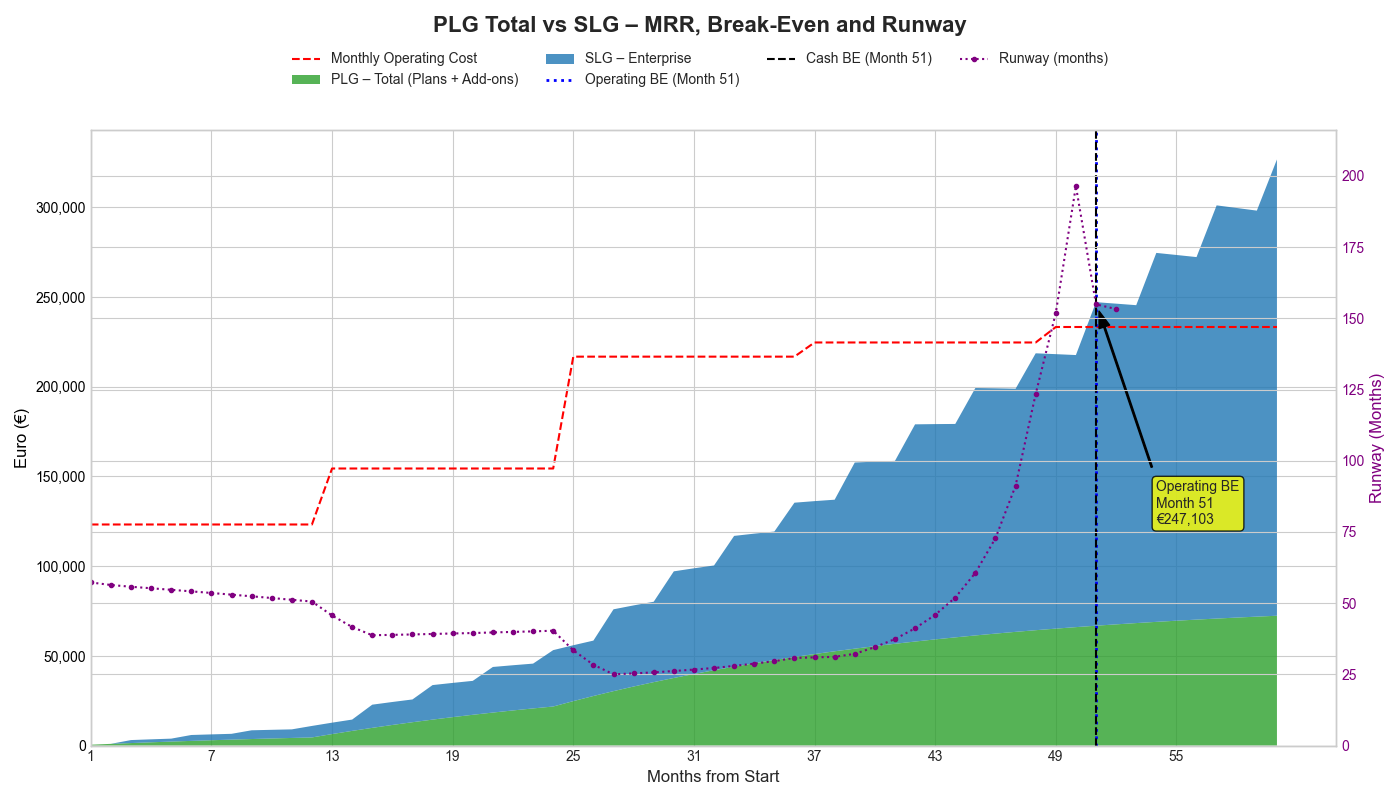
\includegraphics[width=\textwidth]{financial_projection.png}
    \caption{盈亏平衡分析:PLG与SLG MRR、月度成本和营运资金}
    \label{fig:break_even_analysis}
\end{figure} 
\subsection{盈亏平衡分析:图表解读}

\paragraph{图例(快速阅读)}
\begin{itemize}
  \item \textbf{绿色(PLG -- 产品+附加组件):}自助式经常性收入。
  \item \textbf{蓝色(SLG -- 企业):}企业经常性收入;由于年度合同在季度内平滑,因此以季度“阶梯”增长。
  \item \textbf{红色虚线:}月度运营成本(包含谨慎的增长因素),每年以阶梯式增长。
  \item \textbf{紫色点线:}营运资金(月份),计算为现金除以3个月移动平均烧钱额。
  \item \textbf{垂直线:}运营盈亏平衡点(蓝色,51个月)和现金盈亏平衡点(黑色,51个月)。
\end{itemize}

图表显示,前三年公司发展稳健。绿色PLG区域随着每月注册用户(扣除流失后)的复合增长和附加组件带来的增量MRR而稳步上升。蓝色SLG区域在签订企业合同的季度以可见的阶梯式增长。成本呈块状移动:每新增一年,就会增加计划产能(团队、基础设施、一般及管理费用,并包含增长因素),因此红线跳跃然后保持平稳,直到下一个阶梯。

这些动态与年终数据相符。第一年末,成本为\textbf{€123{,}212}/月,而经常性MRR为\textbf{€10{,}948}/月(亏损\textbf{€112{,}149}/月,现金\textbf{€5{,}740{,}147},营运资金\textbf{50.6}个月)。第二年末:\textbf{€154{,}413}对比\textbf{€53{,}194}(亏损\textbf{€100{,}855}/月),现金\textbf{€4{,}282{,}549},营运资金\textbf{40.3}个月。第三年末:\textbf{€216{,}746}对比\textbf{€135{,}360}(亏损\textbf{€80{,}631}/月),现金\textbf{€2{,}239{,}361},营运资金\textbf{30.8}个月。收入曲线明显缩小了与成本的差距,同时现金得到控制:\textbf{观察到的最低营运资金为25.0个月},\textbf{峰值月度烧钱额}为\textbf{€160{,}442}。

第四年,差距显著缩小。较大的SLG阶梯使蓝色区域更快扩张,并且(PLG+SLG)的总和几乎达到成本线。年终:成本\textbf{€224{,}646}/月,经常性MRR为\textbf{€218{,}614}/月(总收入\textbf{€219{,}615}/月),接近持平的亏损为\textbf{€5{,}031}/月,现金\textbf{€2{,}239{,}361}。紫色营运资金线开始飙升,因为移动平均烧钱额接近于零。

% ----- End of translated content from: part_15.tex -----

% ----- Start of translated content from: part_16.tex -----

盈亏平衡点出现在\textbf{第51个月}。此时\textbf{经常性MRR为€247{,}103},而成本为\textbf{€233{,}271}(运营盈亏平衡点),\textbf{总收入€248{,}159}超过成本(现金盈亏平衡点)。为了达到这个目标,该模型\textbf{总共消耗€4{,}939{,}370},\textbf{最低现金}为\textbf{€2{,}234{,}573},这也代表着\textbf{盈亏平衡时的储备(占融资轮的30.9\%)}。到第5年末,经常性MRR达到\textbf{€326{,}645/月}($\approx$ \textbf{€3.92M ARR}),月利润为\textbf{€94{,}565},现金为\textbf{€2{,}673{,}539},并且运营期实际上变得无限长。

\paragraph{要点}
图表清楚地表明了三件事:
\begin{enumerate}
\item \emph{谁推动什么} PLG构建基础,SLG弥补差距
\item \emph{成本为何飙升} 谨慎的提升,伴随着深思熟虑的产能扩张
\item \emph{现金如何保持安全} 运营期从未崩溃(最低25.0个月),并且随着收入超过成本而加速增长,这与打印的指标报告完全一致。
\end{enumerate}

\begin{table}[H]
\centering
\caption{财务预测摘要(年末)}
\label{tab:financial_summary}
\resizebox{\textwidth}{!}{
\begin{tabular}{lrrrrrrr}
\toprule
\textbf{年末} & \textbf{月度成本(€)} & \textbf{经常性MRR(€)} & \textbf{商店收入(€)} & \textbf{总收入(€)} & \textbf{月度损益(€)} & \textbf{现金余额(€)} & \textbf{运营期(月)} \\
\midrule
第1年 & 123,212 & 10,948 & 116 & 11,064 & -112,149 & 5,740,147 & 50.6 \\
第2年 & 154,413 & 53,194 & 364 & 53,558 & -100,855 & 4,282,549 & 40.3 \\
第3年 & 216,746 & 135,360 & 755 & 136,115 & -80,631 & 2,823,198 & 30.8 \\
第4年 & 224,646 & 218,614 & 1,001 & 219,615 & -5,031 & 2,239,361 & 123.5 \\
第5年 & 233,271 & 326,645 & 1,191 & 327,836 & 94,565 & 2,673,539 & 收益状态 \\
\bottomrule
\end{tabular}
}
\end{table}

\begin{table}[H]
\centering
\caption{关键财务指标}
\label{tab:financial_metrics}
\resizebox{\textwidth}{!}{%
\begin{tabular}{ll}
\toprule
\textbf{指标} & \textbf{数值} \\
\midrule
运营盈亏平衡点 & 第51个月(第5年):经常性MRR €247,103 $\geq$ 成本 €233,271 \\
盈亏平衡点 & 第51个月(第5年):总收入 €248,159 $\geq$ 成本 €233,271 \\
达到现金盈亏平衡点前已消耗资本 & €4,939,370 \\
月度峰值消耗 & €160,422 \\
期间最低现金 & €2,210,630(占融资轮的30.9\%) \\
最低运营期(3个月移动平均) & 25.0个月 \\
\bottomrule
\end{tabular}
}
\end{table}

\newpage
\section{为什么CNY 59{,}829{,}055是合适的金额}

我们请求\textbf{CNY 59{,}829{,}055} ($\approx€7.15\text{M}$)是因为这正是根据我们\emph{保守}的预测,能够使公司在\textbf{第51个月达到运营和现金盈亏平衡点}的资金量,同时不会强求增长,并保留具体的安全边际。模拟结果明确显示:\textbf{达到现金盈亏平衡点前累计消耗=€4{,}939{,}370},\textbf{盈亏平衡时的现金余额=€2{,}210{,}630}(即\textbf{30.9\%}的融资轮),\textbf{期间最低运营期=25.0个月}(3个月移动平均),\textbf{月度峰值消耗=€160{,}422}。我们请求的金额是模型显示的\emph{必要且充分}达到盈亏平衡点并具备结构性应急缓冲的金额。

该计划旨在具有韧性:成本并非“精简到极致”,而是按类别(基础设施、一般及管理费用、PLG、SLG、研发、管理)\textbf{谨慎上调},以捕捉经常被低估的经常性项目(企业支持、审计、法律、招聘、监控)。此外,该模型引入了\textbf{自动防护措施}:如果运营期降至12个月以下,则下个月\textbf{酌情成本将削减10\%};如果降至9个月以下,则\textbf{付费PLG收购将被抑制}(乘数0.7)。这些是在模型中编码的操作规则,而不是承诺。实际上,通过自行触发的机制来保护下行风险。

在收入方面,我们清楚地区分\textbf{PLG}(计划+附加组件)和\textbf{SLG}(企业)。这并非形式上的:它让我们能够逐月查看支出杠杆的回报情况,并在没有意识形态的情况下进行再平衡。通过这种组合和当前价格,\textbf{运营盈亏平衡点}出现在\textbf{第51个月},\textbf{经常性MRR为€247{,}103},而\textbf{月度成本为€233{,}271};在同一个月,由于\textbf{总收入(€248{,}159)}超过成本,因此实现了\textbf{现金盈亏平衡点}。到第5年末,经常性MRR达到\textbf{€326{,}645}($\approx$ \textbf{€3.92M ARR})。就资本效率而言,\textbf{隐含的消耗倍数}(盈亏平衡点前的消耗÷盈亏平衡点时的ARR)为\textbf{~1.66倍},这与保守的产品+市场营销策略以及已经可靠上调的成本相符。

那么,为什么是\emph{这个}金额,而不是更少?如果资金较少,则模型将更频繁地触发防护措施,从而造成运营上的走走停停(削减/冷却期),这会延长时间表并提高机会成本,尤其是在连续性至关重要的时候。为什么不多?因为超过这个门槛,瓶颈就不是预算,而是\textbf{渠道吸收能力}和企业交付的自然节奏;今天的额外现金会在不改善模型相对结果的情况下增加稀释。

\textbf{资金用途}仍然与模拟中的各个类别及其上调保持一致:产品/研发(强化、可观察性、安全)、基础设施和企业支持、SLG(账户、解决方案/概念验证)、PLG(内容/SDK/社区)、合作伙伴支持、一般及管理费用和合规性、管理。我们不会开设新的支出项目:我们正在为模型每月衡量的项目提供资金。

最后,\textbf{风险状况}是可读的。最低运营期不会低于\textbf{25.0个月},防护措施会在需要时限制现金流失,而盈亏平衡点的\textbf{30.9\%}缓冲为采购延迟、基础设施/合规支出波动或汇率波动提供了空间。同时,PLG/SLG分离使得直接展示资本配置遵循实际回报,而不是一刀切的计划——即使事后也是如此。

\textbf{简而言之:}\textbf{CNY 59{,}829{,}055}可以充分为达到盈亏平衡点的保守路径提供资金,并具有足够的缓冲和自动成本控制机制。这是一个成比例的、可辩护的,而且最重要的是\textbf{可复制}的要求:投资者可以逐月验证模型指标是否得到控制,以及现金是否遵循预期的轨迹。

\subsection{战略缓冲理由:驾驭AI编排领域的先机}
盈亏平衡点时的30.9\%资本储备(€2.21M)代表着一种深思熟虑的战略配置,用于应对AI编排市场前所未有的变化速度。与产品市场匹配遵循可预测模式的传统SaaS领域不同,AI基础设施领域每3-6个月都会经历根本性的变化——从新的LLM架构到新兴的编排标准,如MCP。该储备使IntellyHub能够快速进行战略调整,而不会影响运营期:无论是适应自主代理能力的突破,整合计划时不存在的具有颠覆意义的模型,还是根据实际市场反应在PLG和SLG渠道之间转移重点。成功的AI基础设施公司(Weights \& Biases、Hugging Face)的历史先例表明,该领域的赢家在实现可持续增长之前需要进行2-3次重大调整——每次都会消耗15-20\%的可用资金。我们的储备确保我们能够在保持12个月以上的运营期的同时执行至少一次重大的战略调整,将原本的生存威胁转变为竞争优势。这不是多余的资金;这是在市场中计算出的可选性保险,在这个市场中,唯一确定的是根本性的变化,而比竞争对手更快地调整方向的能力——当他们争夺紧急资金时——成为市场领导地位和淘汰之间决定性因素。

\newpage
\section{市场营销策略}
% Come raggiungerai i tuoi clienti?

IntellyHub的市场营销策略基于混合模式,结合了两个增长引擎:
\begin{enumerate}
    \item \textbf{面向SaaS的产品主导型增长(PLG):} 我们利用产品的优越性、免费层和自动化商店以可扩展的、自下而上的方式吸引、激活和转化用户。
    \item \textbf{面向本地部署和企业的销售主导型增长(SLG):} 我们采用有针对性的、咨询式的销售方法来赢得具有复杂安全和治理需求的大客户。
\end{enumerate}
这两个引擎旨在相互促进:PLG模式的成功为销售团队创造了潜在客户和品牌知名度。

% ----- End of translated content from: part_16.tex -----

% ----- Start of translated content from: part_17.tex -----

% --- 战略目标 ---
\subsection{战略目标 (三年期)}
\begin{itemize}
    \item \textbf{定位:} 成为领先的平台,为现代技术团队编排复杂的自动化和 AI 工作流。
    \item \textbf{采用率:} 实现活跃用户的临界质量,并在插件生态系统和自动化商店周围建立一个充满活力的社区。
    \item \textbf{收入:} 建立一个可持续的商业模式,拥有可观的年度经常性收入 (ARR),这将由 SaaS 订阅和企业内部部署合同共同驱动。
\end{itemize}

% --- 第一年 ---
\subsection{第一年:基础建设与市场验证}
\textbf{主要重点:} 赢得早期采用者,验证产品市场匹配度,并获得首批关键参考客户(SaaS 和内部部署)。在这个阶段,许多活动是手动的,并且“无法扩展”。

\newpage
\begin{table}[H]
\centering
\resizebox{\textwidth}{!}{
\begin{tabularx}{\textwidth}{L L L} 
\toprule
\textbf{关键渠道} & \textbf{具体行动} & \textbf{成功关键绩效指标} \\

\midrule
\textbf{产品主导增长 (PLG)} & 
\textbf{利基市场发布:} 在 Product Hunt、Hacker News 和相关的技术 subreddits(例如 r/devops、r/kubernetes)等平台上展示 IntellyHub。\newline\newline
\textbf{自动化商店:} 使用 20-30 个高质量的官方模板填充商店,这些模板可以解决实际的、棘手的问题。
&
\textbf{激活率:} >25\%(用户在 7 天内运行其第一个自动化)。\newline\newline
\textbf{1 个月留存率:} >15\%(用户在 4 周后返回)。
\\
\addlinespace

\textbf{技术内容营销} & 
\textbf{博客和教程:} 每月发布 2-4 篇深入的技术文章,展示如何使用 IntellyHub 解决特定问题。\newline\newline
\textbf{视频内容:} 创建简洁的视频教程。
&
\textbf{合格流量:} 来自有机和推荐渠道的网站访问量。\newline\newline
\textbf{访客转化率:} >2\%。
\\
\addlinespace

\textbf{社区建设} &
\textbf{Discord/Slack 频道:} 为早期用户建立一个中心枢纽。\newline\newline
\textbf{创始人主导的支持:}  亲自回答每一个问题和反馈请求,以建立牢固的关系。
&
\textbf{社区参与度:} 每周活跃会员,点对点支持互动。\newline\newline
\textbf{定性反馈:} 每月至少进行 5 次深入的用户访谈。
\\
\addlinespace

\textbf{创始人主导的销售(内部部署)} &
\textbf{利用网络:} 创始人亲自管理来自他们自己网络的目标公司的前 3-5 个销售流程。\newline\newline
\textbf{概念验证 (POC):}  关注一些高价值 POC 的成功。
&
\textbf{启动的 POC:} 全年 3-5 个。\newline\newline
\textbf{签署的内部部署合同:} 1-2 个关键参考客户。
\\
\bottomrule
\end{tabularx}
}
\end{table}


% --- 第二年 ---
\newpage
\subsection{第二年:扩张与建立可重复的增长引擎}
\textbf{主要重点:} 将初始价值转化为可扩展、可重复的流程。优化第一年有效的方法,并建立商业团队的基础。

\begin{table}[H]
\small
\centering
\resizebox{\textwidth}{!}{
\begin{tabularx}{\textwidth}{L L L}
\toprule
\textbf{关键渠道} & \textbf{具体行动} & \textbf{成功关键绩效指标} \\
\midrule
\textbf{PLG 优化} &

\textbf{漏斗分析:} 使用分析工具来识别和消除用户旅程中从注册到付费转化的摩擦点。
\textbf{引导式入门:} 实施应用内入门体验,引导新用户找到他们的“Aha!”时刻。
&

% ----- End of translated content from: part_17.tex -----

% ----- Start of translated content from: part_18.tex -----

\textbf{免费转付费转化率:} >3\%。
\textbf{月均经常性收入 (MRR)增长率:}  连续月度增长。
\\
\addlinespace
\textbf{生态系统合作伙伴关系} &

\textbf{战略集成:} 主动为2-3个具有相似用户群的互补技术平台开发插件。
\textbf{联合营销:} 与合作伙伴开展联合营销活动(网络研讨会、博客文章)。
&

\textbf{合作伙伴提供的潜在客户。}
\textbf{合作伙伴插件下载量。}
\\
\addlinespace
\textbf{初始销售团队} &

\textbf{首批招聘:}  招聘另一名客户主管来处理潜在客户,并开始有针对性的外部勘探。
\textbf{销售策略手册:}  根据创始人领导的销售阶段的经验,规范销售流程。
&

\textbf{每月合格演示次数。}
\textbf{平均销售周期长度(本地部署)。}
\\
\bottomrule
\end{tabularx}
}
\end{table}

\newpage
% --- YEAR 3 ---
\subsection{第三年:规模化与细分市场领导地位}
\textbf{主要目标:} 加速增长,主导技术团队细分市场,并将IntellyHub确立为AI编排市场上的思想领袖。

\begin{table}[H]
\centering
\resizebox{\textwidth}{!}{
\begin{tabularx}{\textwidth}{L L L}
\toprule
\textbf{关键渠道} & \textbf{具体行动} & \textbf{成功关键绩效指标 (KPI)} \\
\midrule
\textbf{销售规模化} &

\textbf{团队扩张:}  扩大销售团队以覆盖不同的地理区域或行业垂直领域。
\textbf{间接渠道:}  开始探索与系统集成商和经销商的合作。
&

\textbf{年度经常性收入 (ARR)增长。}
\textbf{客户获取成本 (CAC) 和 LTV/CAC 比率。}
\\
\addlinespace
\textbf{品牌营销} &

\textbf{思想领导力:}  基于汇总的平台数据发布行业报告。
\textbf{赞助:}  赞助DevOps和AI领域的重点会议和播客。
&

\textbf{行业媒体提及。}
\textbf{直接和品牌流量增长。}
\\
\addlinespace
\textbf{网络效应} &

\textbf{开放商店:}  开放自动化商店和插件市场,以接纳外部贡献的认证合作伙伴。
\textbf{开发者计划:}  启动正式的开发者关系 (DevRel) 计划。
&

\textbf{社区创建的插件/模板数量。}
\textbf{净收入留存率 (NRR):}>110\%。
\\
\bottomrule
\end{tabularx}
}
\end{table}

\clearpage
\section{运营计划}
% Come funzionerà l'azienda giorno per giorno.
\subsection{引言}
本文件概述了执行IntellyHub的开发和市场营销战略的运营计划。该计划与产品开发路线图的各个阶段相一致,并描述了公司各个职能部门的关键活动。

% ----- End of translated content from: part_18.tex -----

% ----- Start of translated content from: part_19.tex -----

% --- 第一阶段 ---
\subsection{第一阶段:基础建设与验证 (第一季度-第二季度)}
\textbf{战略目标:} 将原型转化为稳定安全的最小可行产品 (MVP),获取首批早期用户,并\textbf{通过有针对性的合作伙伴计划验证核心产品和定价模型假设。}

\subsubsection{产品开发与工程}
\begin{itemize}[leftmargin=*]
    \item \textbf{第一季度:}
    \begin{itemize}
        \item \textbf{稳定性:} 完成测试套件(单元测试、集成测试),确保核心引擎的可靠性。
        \item \textbf{插件:} 完成并记录内部系统,以支持标准化插件开发。
        \item \textbf{UI/UX:} 优化混合IDE界面,解决任何同步问题并改善用户体验。
        \item \textbf{本地部署:} 为企业客户开发和测试平台的本地部署版本。
    \end{itemize}
    \item \textbf{第二季度:}
    \begin{itemize}
        \item \textbf{身份验证:} 实施强大的用户管理和身份验证系统。
        \item \textbf{用户引导:} 为新用户开发一个引导式入门向导。
        \item \textbf{自动化商店 (v1): } 创建自动化商店第一版 (只读) 的API和UI。
    \end{itemize}
\end{itemize}

\subsubsection{市场营销 (市场营销与销售)}
\begin{itemize}[leftmargin=*]
    \item \textbf{第一季度-第二季度:}
    \begin{itemize}
        \item \textbf{垂直策略:} 在\textit{初始垂直细分市场}(例如,基于Esplorado的用户案例的生物技术/科学研究)中定义详细的理想客户画像 (ICP)。
        \item \textbf{(新的) 设计合作伙伴计划:} 为目标垂直领域中 3-5 家选定公司启动一个独家计划。提供抢先体验和直接支持,以换取持续反馈和潜在的初步合同。
    \end{itemize}
    \item \textbf{第三季度-第四季度:}
    \begin{itemize}
        \item \textbf{细分市场发布:} 在Product Hunt、Hacker News和相关渠道上执行发布,并将沟通重点放在选择的垂直领域。
        \item \textbf{反馈收集:} 收集免费层用户和(优先)设计合作伙伴的结构化反馈。
    \end{itemize}
\end{itemize}

\subsubsection{社区与生态系统管理}
\begin{itemize}[leftmargin=*]
    \item \textbf{第一季度-第二季度:}
    \begin{itemize}
        \item \textbf{有针对性的插件开发:} 开发并记录第一个“官方”插件,\textit{优先考虑与目标垂直领域最相关的插件}。
    \end{itemize}
    \item \textbf{第三季度-第四季度:}
    \begin{itemize}
        \item \textbf{社区创建:} 启动官方Discord/Slack服务器。
        \item \textbf{参与度:} 创始人及开发团队将积极参与,解答问题并营造友好的环境。
    \end{itemize}
\end{itemize}

\subsubsection{一般及公司运营}
\begin{itemize}[leftmargin=*]
    \item \textbf{第一季度-第二季度:}
    \begin{itemize}
        \item \textbf{法律和行政设置:} 完成公司结构搭建,开设银行账户。
        \item \textbf{(新的) 合作伙伴签约:} 为“设计合作伙伴计划”准备协议。
    \end{itemize}
    \item \textbf{第三季度-第四季度:}
    \begin{itemize}
        \item \textbf{服务条款定义:} 为免费层发布撰写和发布服务条款和隐私政策。
    \end{itemize}
\end{itemize}

\clearpage

% --- 第二阶段 ---
\subsection{第二阶段:扩张与增长 (第三季度-第四季度)}
\textbf{战略目标:} 基于第一阶段验证的数据,扩展用户获取规模,扩展生态系统,并实施必要的企业级功能以实现盈利。

\subsubsection{产品开发与工程}
\begin{itemize}[leftmargin=*]
    \item \textbf{第五季度-第六季度:}
    \begin{itemize}
        \item \textbf{安全性:} 为凭据实施密钥管理系统。
        \item \textbf{版本控制:} 为自动化流程添加历史记录和回滚功能。
    \end{itemize}
    \item \textbf{第七季度-第八季度:}
    \begin{itemize}
        \item \textbf{可观察性:} 开发数据平台的第一个版本,用于流程性能指标。
        \item \textbf{改进仪表盘:} 创建用于可视化流程的用户界面。
        \item \textbf{主动式AI:} 基于流程性能数据实施基本的“自动修复”功能。
    \end{itemize}
\end{itemize}

\subsubsection{市场推广(市场营销与销售)}
\begin{itemize}[leftmargin=*]
    \item \textbf{Q5-Q6:}
    \begin{itemize}
        \item \textbf{垂直内容营销:} 扩大内容制作规模(基于设计合作伙伴的案例研究、文章),重点关注所选垂直领域。
        \item \textbf{招聘:} 开始招聘首位开发者布道师。
    \end{itemize}
    \item \textbf{Q7-Q8:}
    \begin{itemize}
        \item \textbf{付费计划发布:} 完成定价(已通过设计合作伙伴验证)并正式发布专业版和企业版计划。
        \item \textbf{销售策略手册(v1):} 开始为企业客户记录销售流程。
    \end{itemize}
\end{itemize}

\clearpage

% --- PHASE 3 ---
\subsection{第三阶段:领导力和创新(第5-6季度)}
\textbf{战略目标:} 建立市场领导地位,通过社区效应创造网络效应,并\textbf{利用数据建立难以逾越的竞争优势。}

\subsubsection{产品开发与工程}
\begin{itemize}[leftmargin=*]
    \item \textbf{Q9-Q10:}
    \begin{itemize}
        \item \textbf{商店开放:} 开放商店,允许社区提交内容。
        \item \textbf{审核:} 实施内部工具,用于审核和验证外部贡献。
    \end{itemize}
    \item \textbf{Q11-Q12:}
    \begin{itemize}
        \item \textbf{(修订版)数据平台与可观察性:} 开发用于收集和聚合流量性能指标的系统,战略目标是\textbf{构建“数据护城河”。}
        \item \textbf{分析仪表板:} 创建用于可视化分析的用户界面。
        \item \textbf{主动式AI:} 改善“自动修复”和主动优化功能,\textbf{基于聚合的平台数据进行训练。}
    \end{itemize}
\end{itemize}

\subsubsection{市场推广(市场营销与销售)}
\begin{itemize}[leftmargin=*]
    \item \textbf{Q9-Q10:}
    \begin{itemize}
        \item \textbf{销售团队扩展:} 聘请更多客户主管来覆盖特定市场或垂直领域。
        \item \textbf{思想领导力:} 开始发布基于平台使用数据的报告和分析。
    \end{itemize}
    \item \textbf{Q11-Q12:}
    \begin{itemize}
        \item \textbf{品牌营销:} 增加对品牌知名度活动的投资(赞助、活动)。
    \end{itemize}
\end{itemize}

\newpage
\section{风险分析}
\subsection{市场风险}
\textit{与市场、竞争和客户采用相关的风险。}

\begin{table}[H]
\centering
\begin{tabularx}{\textwidth}{@{}lL@{}}
\toprule
\textbf{风险} & \textbf{描述} \\
\midrule
\textbf{来自“现状”的竞争} & 我们最大的竞争对手不是另一个平台,而是开发者使用自定义Python脚本的惯性。他们对它的熟悉程度以及看似为零的初始成本使其成为一个需要克服的重大障碍。 \\
\addlinespace
\textbf{企业采用周期缓慢} & 内部部署和企业销售模式对于高价值合同至关重要,但其特点是销售周期长(6-12个月以上)且概念验证(POC)阶段复杂。延迟达成首笔关键企业交易可能会严重影响收入预测。 \\
\addlinespace
\textbf{AI技术转变} & 我们目前的AI定位为“副驾驶”。如果竞争对手在真正自主的、“足够好”的AI代理方面取得快速的技术飞跃,可能会使我们更受控制、更有结构化的方法显得不那么创新。 \\
\bottomrule
\end{tabularx}
\end{table}

\newpage
\subsection{运营风险}
\textit{与技术、人员和执行相关的风险。}

\begin{table}[H]
\centering
\begin{tabularx}{\textwidth}{@{}lL@{}}
\toprule
\textbf{风险} & \textbf{描述} \\

% ----- End of translated content from: part_20.tex -----

% ----- Start of translated content from: part_21.tex -----

\midrule
\textbf{团队执行与关键人员风险} & 该计划依赖于聘用少量高度专业化的个人。项目的成功高度依赖于核心团队在产品、基础设施和销售方面的执行能力。关键成员的离职可能会导致严重的延误。 \\
\addlinespace
\textbf{技术复杂性} & 技术栈(Kubernetes、多步骤AI管道、混合IDE)功能极其强大,但也难以维护和发展。这个复杂系统中的错误、安全漏洞或性能瓶颈可能难以且代价高昂地解决。 \\
\addlinespace
\textbf{混合技术风险(IDE/YAML同步)} & 维持复杂可视化IDE与文本YAML表示之间完美的、实时的、双向同步在技术上极具挑战性。这是潜在的、难以调试的细微错误的来源,可能会影响用户信任。 \\
\addlinespace
\textbf{生态系统质量控制} & 自动化商店和插件市场的价值是一把双刃剑。低质量的、不安全的或维护不善的社区贡献可能会损害用户信任和平台声誉。 \\
\bottomrule
\end{tabularx}
\end{table}

\newpage
\subsection{财务风险}
\textit{与现金流、资金和财务可持续性相关的风险。}

\begin{table}[H]
\centering
\begin{tabularx}{\textwidth}{@{}lL@{}}
\toprule
\textbf{风险} & \textbf{描述} \\
\midrule
\textbf{高初始资金消耗率} & 激进的招聘计划导致在产生可观收入之前产生高昂的每月运营成本。这给快速实现产品市场匹配和产生收入带来了巨大压力。 \\
\addlinespace
\textbf{资金依赖} & 商业模式并非旨在追求短期盈利。未能达到投资者预期的增长KPI将构成生存威胁。 \\
\addlinespace
\textbf{定价模式验证} & 提出的价值指标(执行次数、活跃自动化)合乎逻辑,但尚未经过验证。错误的定价模式可能导致客户摩擦(如果价格过高)或遗漏大量收入(如果价格过低)。 \\
\bottomrule
\end{tabularx}
\end{table}

\newpage
\subsection{缓解策略}
\textit{解决和降低已识别风险的具体措施。}

\begin{table}[H]
\centering
\begin{tabularx}{\textwidth}{@{}lL@{}}
\toprule
\textbf{风险类别} & \textbf{缓解策略} \\
\midrule
\textbf{市场风险} & 
\textbf{定位与教育:}将营销重点放在消除管理\textit{大量}脚本的长期混乱上,而不是仅仅替换单个脚本。使用诸如“Esplorado”之类的案例研究来提供无可辩驳的价值证明。 \newline\newline
\textbf{混合市场进入策略:}同时运行PLG(SaaS)和SLG(本地部署)模式。利用PLG侧更快的反馈循环来改进针对较慢的企业销售周期的产品和信息。 \newline\newline
\textbf{战略性AI路线图:}将当前的AI定位为生产环境中实用、安全可靠的选择。将路线图定义为朝着更自主能力发展的演变,建立在我们今天拥有的强大基础之上。 \\
\addlinespace
\textbf{运营风险} & 
\textbf{文档与交叉培训:}从第一天起就大力投资内部文档。实施知识共享和结对编程文化,以减少对个人的依赖。 \newline\newline
\textbf{投资可观察性和测试:}将资源专门用于强大的自动化测试套件,并在早期集成APM(应用程序性能监控)工具,以主动识别和解决问题。测试套件专门涵盖IDE/YAML同步逻辑。 \newline\newline
\textbf{精心策划的生态系统:}最初,商店只将展示“官方”和“验证合作伙伴”插件。对所有未来的社区提交实施清晰而严格的审查流程,包括自动安全扫描和质量检查。 \\
\addlinespace
\textbf{财务风险} & 
\textbf{基于里程碑的支出:}将支出的大幅增加(尤其是在营销和销售人员招聘方面)与实现特定预定义的里程碑(例如,达到前10个付费客户,实现一定的留存率)联系起来。 \newline\newline
\textbf{持续的投资者关系:}与现有和潜在的未来投资者保持透明和定期的沟通渠道,分享KPI的进展,以建立信心并简化下一轮融资。 \newline\newline
\textbf{价格迭代:}采用简单灵活的定价模式启动。直接与早期客户互动,了解他们获得的价值,并准备根据他们的反馈和使用数据迭代定价结构。 \\
\bottomrule
\end{tabularx}
\end{table}

\newpage
% \subsection{产品截图}
% 产品的截图、模型图或图表。

\newpage
% 在此处添加文档中引用的任何来源、研究或文章。
\begin{thebibliography}{99}
    \bibitem{AIMarket}
    Market.us,《自动化机器学习市场报告》,网址:\url{https://market.us/report/automated-machine-learning-market/}, 2025年3月。
    
    \bibitem{MLOpsMarket}
    MarketReserchFuture.com,《MLOps市场研究报告:按组件(服务、平台)、按部署模式(本地部署、云)、按组织规模(大型企业、中小型企业)、按垂直行业(BFSI、零售和电子商务、政府和国防、医疗保健和生命科学、制造业等)和按地区(北美、欧洲、亚太地区和世界其他地区)划分的市场预测,直至2034年。》,网址:\url{https://www.marketresearchfuture.com/reports/mlops-market-18849}, 2025年8月。
    
    \bibitem{AIOrch}
    Market.us,《AI编排平台市场报告(2024-2034年预测)》,2025年2月。网址:\url{https://market.us/report/ai-orchestration-platform-market/}。

    \bibitem{GartnerAgentic}
    路透社(报道Gartner),《超过40%的自主AI项目将在2027年前被取消……到2028年,33%的企业软件将包含自主AI,15%的决策将由自主系统做出》,2025年6月25日。网址:\url{https://www.reuters.com/business/over-40-agentic-ai-projects-will-be-scrapped-by-2027-gartner-says-2025-06-25/}。


    \bibitem{MLOpsMM}
    MarketsandMarkets Research,\textit{MLOps市场规模预计到2027年将超过59亿美元,复合年增长率为41.0\%},2023年4月21日。
    网址:\url{https://www.globenewswire.com/news-release/2023/04/21/2652028/0/en/MLOps-Market-Size-is-Anticipated-to-Cross-US-5-9-billion-by-2027-growing-at-a-CAGR-of-41-0-Report-by-MarketsandMarkets.html}.

    \bibitem{ModelOpsGV}
    Grand View Research,\textit{ModelOps市场报告},2025年版。
    网址:\url{https://www.grandviewresearch.com/industry-analysis/modelops-market-report}.

    \bibitem{AIMLMarket}
    Market.us,\textit{自动化机器学习市场报告(2024-2034年预测)},2025年3月。
    网址:\url{https://market.us/report/automated-machine-learning-market/}.

    \bibitem{MLOpsMRF}
    MarketResearchFuture,\textit{MLOps市场研究报告(2024-2034年预测)},2025年8月。
    网址:\url{https://www.marketresearchfuture.com/reports/mlops-market-18849}.

    \bibitem{deloitte2020}
    德勤,\textit{智能边缘自动化:超级企业的新疆界},2020年。
    网址:\url{https://www2.deloitte.com/us/en/insights/topics/talent/intelligent-automation-2020-survey-results.html}

    \bibitem{grandviewRPA}
    Grand View Research,\textit{机器人流程自动化(RPA)市场规模、份额和趋势分析报告},2024年。
    网址:\url{https://www.grandviewresearch.com/industry-analysis/robotic-process-automation-rpa-market}

    \bibitem{mckinseyAI2023}
    麦肯锡公司,\textit{2023年人工智能现状:生成式人工智能的突破之年},2023年8月1日。
    网址:\url{https://www.mckinsey.com/capabilities/quantumblack/our-insights/the-state-of-ai-in-2023-generative-ais-breakout-year}


    \bibitem{langchainGitHub}
    LangChain GitHub代码库。
    网址:\url{https://github.com/langchain-ai/langchain}

    \bibitem{gartnerAIBarriers}
    Gartner,\textit{人工智能应用的两个障碍},2021年11月2日。
    网址:\url{https://www.gartner.com/en/articles/2-barriers-to-ai-adoption}

    \bibitem{euAIAct}
    欧盟委员会,\textit{关于人工智能的监管框架提案}。
    网址:\url{https://digital-strategy.ec.europa.eu/en/policies/regulatory-framework-ai}

    \bibitem{AIOrch}
    Market.us,\textit{AI编排平台市场报告(2024-2034年预测)},2025年2月。
    网址:\url{https://market.us/report/ai-orchestration-platform-market/}.

    \bibitem{zapierApps}
    Zapier,\textit{探索6000多个应用程序}。
    网址:\url{https://zapier.com/apps}

    \bibitem{g2ZapierReviews}
    G2,\textit{Zapier评论}。
    网址:\url{https://www.g2.com/products/zapier/reviews}

    \bibitem{zapierPricing}
    Zapier,\textit{Zapier定价计划}。
    网址:\url{https://zapier.com/pricing}


    \bibitem{zapierOpenAI}
    Zapier,\textit{OpenAI集成}。
    网址:\url{https://zapier.com/apps/openai/integrations}

    \bibitem{g2MakeVsZapier}
    G2,\textit{比较Make和Zapier}。
    网址:\url{https://www.g2.com/compare/make-vs-zapier}


    \bibitem{autogenGitHub}
    微软,\textit{AutoGen GitHub代码库}。
    网址:\url{https://github.com/microsoft/autogen}

    \bibitem{crewaiGitHub}
    Joao Moura,\textit{CrewAI GitHub代码库}。
    网址:\url{https://github.com/joaomdmoura/crewAI}

    \bibitem{langchainValuation}
    TechCrunch,\textit{据报道,人工智能基础设施初创公司LangChain以11亿美元的估值筹集了1亿美元},2025年7月9日。
    网址:\url{https://siliconangle.com/2025/07/09/ai-infrastructure-startup-langchain-reportedly-raises-100m-1-1b-valuation/#:~:text=Artificial%20intelligence%20infrastructure%2C%20developer%20tools,on%20a%20%241.1%20billion%20valuation.}

    \bibitem{langchainIntegrations}
    LangChain文档,\textit{LangChain集成}。
    网址:\url{https://python.langchain.com/docs/integrations/providers/}

    \bibitem{langchainCritique}
    Medium,\textit{LangChain的挑战与批评},2025年3月3日。
    网址:\url{https://shashankguda.medium.com/challenges-criticisms-of-langchain-b26afcef94e7}

    \bibitem{mrfRPA}
    Market Research Future,\textit{机器人流程自动化(RPA)市场研究报告信息,按流程(决策支持、自动化解决方案和管理解决方案)、按运营(基于规则和基于知识)、按行业(制造与物流以及IT与电信)和按地区(北美、欧洲、亚太地区和世界其他地区)划分——行业规模、份额和预测至2032年}。
    网址:\url{https://www.marketresearchfuture.com/reports/robotic-process-automation-market-2209}

    \bibitem{uipathGartner}
    UiPath,\textit{Gartner RPA魔力象限},2025年。
    网址:\url{https://www.uipath.com/resources/automation-analyst-reports/gartner-magic-quadrant-robotic-process-automation}

    \bibitem{awsSagemaker}
    Amazon AWS SageMaker,\textit{Amazon SageMaker},
    网址:\url{https://aws.amazon.com/sagemaker/}

% ----- End of translated content from: part_22.tex -----

% ----- Start of translated content from: part_23.tex -----

\bibitem{forresterRPAvsAI}
    Craig Le Clair,\textit{RPA平台仍将具有相关性吗?AI智能体或许能给出答案。},Forrester,2024年4月25日。网址:\url{https://www.forrester.com/blogs/will-rpa-platforms-remain-relevant-ai-agents-may-hold-the-answer/}

\end{thebibliography}


\end{document}

% ----- End of translated content from: part_23.tex -----

